\section{Vectors}

\begin{frame}
	\frametitle{Vectors and spatential interpretation}
	\begin{block}{Properties of a vector}
		There are 3 properties of a vector $\overrightarrow{x}$:
		\begin{itemize}
			\item magnitude
			\item direction
			\item start point
		\end{itemize}
		{\bf with respect to} a referention vector $\overrightarrow{0}$
	\end{block}
\end{frame}

\begin{frame}
	\begin{block}{Multiplication between a scalar and a vector}
		r $\in \mathbb{R}$ (r $\in \mathbb{C}$ is possible, but hasn't a physical representation)
		\begin{itemize}
			\item $|r|<1$: short the vector
			\item $|r|>1$: increase the vector
			\item $r<0$: reverse the direction
		\end{itemize}
	\end{block}
	\begin{block}{Addition of vectors}
		Parallelogram rule:

		\begin{figure}
			\centering
			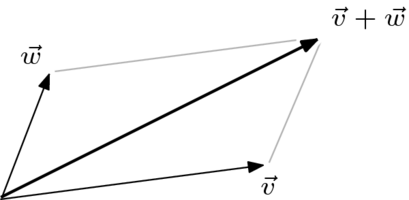
\includegraphics[width=0.4\linewidth]{optelling}
		\end{figure}
	\end{block} 
\end{frame}

\begin{frame}
	\frametitle{Vector spaces}
	\begin{block}{First condition}
		A vector space V over a body L (set of operators) is a set of vectors that satisfy:\\
		1. A vector sum is defined: $VxV\rightarrow V:(\overrightarrow{x},\overrightarrow{y})\rightarrow\overrightarrow{x}+\overrightarrow{y}$\\
		 \hspace{1.5 cm}$\overrightarrow{x}$, $\overrightarrow{y}$, $\overrightarrow{z}$ $\in$ V
		\begin{description}
			\item[a)] $\overrightarrow{x}+\overrightarrow{y}$ $\in$ V
			\item[b)] $\overrightarrow{x}+(\overrightarrow{y}+\overrightarrow{z})=(\overrightarrow{x}+\overrightarrow{y})+\overrightarrow{z}$
			\item[c)] $\exists!\overrightarrow{0}: \overrightarrow{x}+\overrightarrow{0}=\overrightarrow{0}+\overrightarrow{x}=\overrightarrow{x}$
			\item[d)] $\forall \overrightarrow{x}, \exists (-\overrightarrow{x}):\overrightarrow{x}+(-\overrightarrow{x})=(-\overrightarrow{x})+\overrightarrow{x}=0$
			\item[e)] $\overrightarrow{x}+\overrightarrow{y}=\overrightarrow{y}+\overrightarrow{x}$
		\end{description}
	\end{block}
\end{frame}

\begin{frame}
	\frametitle{Vector spaces}
	\begin{block}{Second condition}
		2. A outside law is defined: $LxV\rightarrow V:(a,\overrightarrow{x})\rightarrow a\overrightarrow{x}$\\
		\hspace{1.5 cm}$\overrightarrow{x}$, $\overrightarrow{y}$ $\in$ V\\
		\hspace{1.5 cm}a,b $\in$ L
		\begin{description}
			\item[a)] $1\overrightarrow{x}=\overrightarrow{x}$
			\item[b)] $a(b\overrightarrow{x})=(ab)\overrightarrow{x}$
			\item[c)] $(a+b)\overrightarrow{x}=a\overrightarrow{x}+b\overrightarrow{x}$
			\item[d)] $a(\overrightarrow{x}+\overrightarrow{y})=a\overrightarrow{x}+a\overrightarrow{y}$
		\end{description}
	\end{block} 
\end{frame}

\begin{frame}
	\frametitle{Numberspaces of n-couples}
	\begin{block}{Defenition}
		This is the set of all n-couples 
		$\begin{bmatrix}
			x_1\\
			x_2\\
			.\\
			.\\
			x_n
		\end{bmatrix}$ with $x_i$ $\in$ $\mathbb{R}$ or $x_i$ $\in$ $\mathbb{C}$ (i=1,...,n).\\
		This set together with the operator set $\mathbb{R}$ or $\mathbb{C}$ is a vector space.
	\end{block}
\end{frame}
		
\begin{frame}
	\frametitle{Subspaces}
	\begin{block}{Defenition}
		$V_1$ is a subspace of vector space V if:\\ 
		\begin{enumerate}
			\item $V_1 \subset$ V
			\item With the same in- and outside law as V, is $V_1$ a vector space.
		\end{enumerate}
	\end{block}
	\begin{block}{Properties}
		\begin{enumerate}
			\item $\overrightarrow{0}$ $\in$ every subspace
			\item The intersection of two spaces is always a subspace.
			\item Given: p vectors $\overrightarrow{x_1},\overrightarrow{x_2},...,\overrightarrow{x_p}$ $\in$ V.\\
			The set vectors $a_1\overrightarrow{x_1}+a_2\overrightarrow{x_2}+...+a_p\overrightarrow{x_p}$ with $a_i$ $\in$ $\mathbb{R}$ is a subspace of V.
		\end{enumerate}
	\end{block}
\end{frame}

\begin{frame}
	\frametitle{Linear independence, basis, dimensions}
	\begin{block}{Defenition independence}
		Given: p vectors $\overrightarrow{x_1},\overrightarrow{x_2},...,\overrightarrow{x_p}$ $\epsilon$ V.\\
		Construct the null vector as a linear combination of those vectors (i.e. search the operators (numbers) $a_1,a_2,...,a_p$ to form $a_1\overrightarrow{x_1}+a_2\overrightarrow{x_2}+...+a_n\overrightarrow{x_n}=\overrightarrow{0}$).\\
		If the null vector only can by created by $a_1=a_2=...=a_p=0$, then are the vectors $\overrightarrow{x_1},\overrightarrow{x_2},...,\overrightarrow{x_p}$ {\bf linear independent}.
	\end{block}
\end{frame}

\begin{frame}
	\frametitle{Linear independence, basis, dimensions}
	\begin{block}{Properties linear independence}
		\begin{enumerate}
			\item If the vectors $\overrightarrow{x_1},\overrightarrow{x_2},...,\overrightarrow{x_p}$ are linear independent, then can't none of them be written as a linear combination of the other p-1 vectors.
			\item If the null vector is one of the p vectors, then is the set $\overrightarrow{x_1},\overrightarrow{x_2},...,\overrightarrow{x_p}$ linear dependent (if $\overrightarrow{x_1}=0$ then is $a_1\overrightarrow{x_1}+a_2\overrightarrow{x_2}+...+a_n\overrightarrow{x_n}=0$ with $a_1\neq0$ and $a_2,a_3,...a_p=0$).
			\item Basis and dimension: p linear independent vectors $\overrightarrow{x_1},\overrightarrow{x_2},...,\overrightarrow{x_p}$ generate a vector space $V^p$. Every vector in $V^p$ can be written {\bf in only one way} as a linear combination of the p linear independent vectors $\overrightarrow{x_1},\overrightarrow{x_2},...,\overrightarrow{x_p}$ using operators $a_1,a_2,...,a_p$.
		\end{enumerate}
	\end{block}
\end{frame}

\begin{frame}
	\frametitle{Linear independence, basis, dimensions}
	\begin{block}{Basis, dimension}
		Given: $\overrightarrow{v}=a_1\overrightarrow{x_1}+a_2\overrightarrow{x_2}+...+a_p\overrightarrow{x_p}$.\\
		The set operators \{$a_1,a_2,...,a_p$\} are called the {\bf coordinates} of the vector $\overrightarrow{v}$ relative to the set vectors \{$\overrightarrow{x_1},\overrightarrow{x_2},...,\overrightarrow{x_p}$\}. This set vectors is a {\bf basis} of the vector space $V^p$, with {\bf dimension} p.
	\end{block}
\end{frame}

\begin{frame}
	\frametitle{Linear independence, basis, dimensions}
	\begin{block}{Example}
		Given: $\overrightarrow{x_1}=\begin{bmatrix} 1\\0\\0\end{bmatrix}, \overrightarrow{x_2}=\begin{bmatrix} 0\\1\\0\end{bmatrix}, \overrightarrow{x_3}=\begin{bmatrix} 0\\0\\1\end{bmatrix}$\\
		The set \{$\overrightarrow{x_1},\overrightarrow{x_2},\overrightarrow{x_3}$\} is a linear independent combination. There doesn't exist numbers $a_1\neq0$, $a_2\neq0$, $a_3\neq0$ such that $a_1\overrightarrow{x_1}+a_2\overrightarrow{x_2}+a_n\overrightarrow{x_3}=0$. The set of all vectors $\overrightarrow{y}= a_1\overrightarrow{x_1}+ a_2\overrightarrow{x_2}+ a_n\overrightarrow{x_3}$ is the three dimensional vector space $V^3$.\\
		If $\overrightarrow{y}=\begin{bmatrix} 3\\2\\1\end{bmatrix}$. Then $3\overrightarrow{x_1}+2\overrightarrow{x_2}+\overrightarrow{x_3}$ is the only way to write $\overrightarrow{y}$ as a linear combination of $\overrightarrow{x_1},\overrightarrow{x_2},\overrightarrow{x_3}$.
	\end{block}
\end{frame}

\begin{frame}
	\frametitle{Linear independence, basis, dimensions}
	\begin{block}{Example}
		The set vectors $\overrightarrow{y}=a_1\overrightarrow{x_1}+a_2\overrightarrow{x_2}$ is a {\bf two dimensional} subspace $V^2$.\\
		The vectors in this subspace are: $\overrightarrow{y}=\begin{bmatrix} y_1\\y_2\\y_3\end{bmatrix}=a_1\begin{bmatrix} 1\\0\\0\end{bmatrix}+ a_2\begin{bmatrix} 0\\1\\0\end{bmatrix}=\begin{bmatrix} a_1\\a_2\\0\end{bmatrix}$.
	\end{block}
	\begin{block}{Important difference}
		\begin{itemize}
			\item All vectors of $V^2$ have \textbf{3} coordinates.
			\item The dimension of the subspace $V^2$ is \textbf{2}.
		\end{itemize}
	\end{block}
\end{frame}

\begin{frame}
	\frametitle{Linear independence, basis, dimensions}
	\begin{block}{Convention of notation}
		Given: a n-dimensional vector space $V^n$.\\
		The elements of this vector space are: $\overrightarrow{x},\overrightarrow{y},..$. If we choose $\overrightarrow{e_1},\overrightarrow{e_2},...,\overrightarrow{e_n}$ as a basis of $V^n$, then we can write every vector of $V^n$ as a linear combination of those basis vectors in only one way: $\overrightarrow{x}=x_1\overrightarrow{e_1}+x_2\overrightarrow{e_2}+ ...+x_n\overrightarrow{e_n}$. The numbers $x_i$ are the coordinates of vector $\overrightarrow{x}$ relative to the basis $\overrightarrow{e_1},\overrightarrow{e_2},..., \overrightarrow{e_n}$.\vspace{5mm}
		Between the vector space of dimension n and the number space of dimension n exists a isomorphism.	
	\end{block}
\end{frame}

\begin{frame}
	\frametitle{Linear independence, basis, dimensions}
	\begin{block}{Vector space $V^p$}
		Given: a p-dimensional vector space $V^p$ where the vectors are n-couples (with $n\geq p$).
		\begin{enumerate}
			\item In $V^p$ exists a basis with p linear independent vectors.
			\item Every vector $\overrightarrow{x}$ $\in$ $V^p$ can be written in only one way as a linear combination of the p basis vectors using coordinates.
		\end{enumerate}	
	\end{block}
	\begin{block}{Example 1}
		Given: n=5, p=2, $\overrightarrow{x_1}=\begin{bmatrix} 1\\0\\-1\\2\\5\end{bmatrix}, \overrightarrow{x_2}=\begin{bmatrix} 2\\-3\\1\\0\\0\end{bmatrix}$.\\
	\end{block}
\end{frame}

\begin{frame}
	\frametitle{Linear independence, basis, dimensions}
	\begin{block}{Example 1}
		The vectors $\overrightarrow{x_1}$ and $\overrightarrow{x_2}$ are linear independent, so they span a two dimensional subspace: $\overrightarrow{y}=a_1\overrightarrow{x_1}+a_2\overrightarrow{x_2}$ with $a_1, a_2$ $\in$ $\mathbb{R}$.\\
		The coordinates of the vector $y_1=\begin{bmatrix} 5\\-6\\1\\2\\5\end{bmatrix}$ are $a_1=1$ and $a_2=2$, relative to the basis \{$\overrightarrow{x_1},\overrightarrow{x_2}$\}.
	\end{block}
\end{frame}

\begin{frame}
	\frametitle{Linear independence, basis, dimensions}
	\begin{block}{Example 1}
		The vector $\overrightarrow{y_2}=\begin{bmatrix} 5\\-7\\1\\2\\5\end{bmatrix}$ can't be written as a linear combination of the vectors $\overrightarrow{x_1}$ and $\overrightarrow{x_2}$. So $y_2$ doesn't belong to the subspace spanned by $\overrightarrow{x_1}$ and $\overrightarrow{x_2}$.\\
		This implies that $\overrightarrow{y_2}$ is linear independent with $\overrightarrow{x_1}$ and $\overrightarrow{x_2}$.\\
		 Hence, the subspace spanned by $\overrightarrow{y_2}$, $\overrightarrow{x_1}$ and $\overrightarrow{x_2}$ is a 3 dimensional subspace.
	\end{block}
\end{frame}

\begin{frame}
	\frametitle{Linear independence, basis, dimensions}
	\begin{block}{In general}
		When the set vectors $\overrightarrow{x_1},\overrightarrow{x_2},..., \overrightarrow{x_p}$ is linear independent, then is $\overrightarrow{x_i}$ not totally in the subspace spanned by the vectors $\overrightarrow{x_1},..., \overrightarrow{x}_{i-1}, \overrightarrow{x}_{i+1},...,\overrightarrow{x_p}$.\\
		The vector $\overrightarrow{x_i}$ can be written as a sum of 2 components: $\overrightarrow{x}_{i\alpha}$ and $\overrightarrow{x}_{i\beta}$.
		\begin{enumerate}
			\item $\overrightarrow{x}_{i\alpha}$ $\in$ subspace spanned by $\overrightarrow{x_1},..., \overrightarrow{x}_{i-1}, \overrightarrow{x}_{i+1},...,\overrightarrow{x_p}$.
			\item $\overrightarrow{x}_{i\beta}$ $\bot$ subspace spanned by $\overrightarrow{x_1},..., \overrightarrow{x}_{i-1}, \overrightarrow{x}_{i+1},...,\overrightarrow{x_p}$.
		\end{enumerate}
	\end{block}
\end{frame}

\begin{frame}
	\frametitle{Inner product}
	\begin{block}{Defenition}
		The inner product of two vectors $\overrightarrow{x}$ and $\overrightarrow{y}$ $\in$ $E^n$ (n-couples) is defined as the image: $E^nxE^n\to\mathbb{R}:\{\overrightarrow{x},\overrightarrow{y}\}\to\overrightarrow{x}.\overrightarrow{y}$ $\in$ $\mathbb{R}$. This image is:
		\begin{enumerate}
			\item Bilinear:\\ $(\overrightarrow{x}+\overrightarrow{v}).\overrightarrow{y}=\overrightarrow{x}.\overrightarrow{y}+\overrightarrow{v}.\overrightarrow{y}$\\
			$\overrightarrow{x}(\overrightarrow{v}+\overrightarrow{y})=\overrightarrow{x}.\overrightarrow{v}+\overrightarrow{x}.\overrightarrow{y}$\\
			$(a\overrightarrow{x})\overrightarrow{y}=a(\overrightarrow{x}.\overrightarrow{y})$\\
			$\overrightarrow{x}(a\overrightarrow{y})=a(\overrightarrow{x}.\overrightarrow{y})$
			\item Symmetric:\\
			$\overrightarrow{x}.\overrightarrow{y}=\overrightarrow{y}.\overrightarrow{x}$
			\item Positive definite:\\
			$\forall \overrightarrow{x} \neq \overrightarrow{0}$: $\overrightarrow{x} .\overrightarrow{x} > 0$
		\end{enumerate}
	\end{block}
\end{frame}

\begin{frame}
	\frametitle{Inner product}
	\begin{block}{Matricial notation}
		The inner product is a {\bf scalar}. If $\overrightarrow{x}$, $\overrightarrow{y}$ and the basis $\in$ $E^n$, then can the inner product be noted matricial:\\
		$\overrightarrow{x}.\overrightarrow{y}=y^tAx=x^tAy=(x_1...x_n)A\begin{pmatrix} y_1\\...\\y_n\end{pmatrix}$\\
		with A positive definite and symmetric ($A=A^t$).
	\end{block} 
\end{frame}

\begin{frame}
	\frametitle{Inner product}
	\begin{block}{Norm of a vector}
		$\|\overrightarrow{x}\|^2=\overrightarrow{x}.\overrightarrow{x}$ and because $\overrightarrow{x}.\overrightarrow{x}>0$:\\
		$\|\overrightarrow{x}\|=\sqrt{\overrightarrow{x}.\overrightarrow{x}}$ where $\|\overrightarrow{x}\|$ is called the norm of $\overrightarrow{x}$.\\
		Normalizing is dividing a vector by its norm. The result is a vector with norm $=1$.\\
		$\|\frac{\overrightarrow{x}}{\|\overrightarrow{x}\|}\|= \sqrt{\frac{\overrightarrow{x}}{\|\overrightarrow{x}\|} \frac{\overrightarrow{x}}{\|\overrightarrow{x}\|}}= \sqrt{\frac{\|\overrightarrow{x}\|^2}{\|\overrightarrow{x}\|\|\overrightarrow{x}\|}}=1$.
	\end{block} 
\end{frame}

\begin{frame}
	\frametitle{Inner product}
	\begin{block}{Cauchy Schwarz inequality}
		$|\overrightarrow{x}.\overrightarrow{y}|\leq \|\overrightarrow{x}\|\|\overrightarrow{y}\|$ or \\
		$-\|\overrightarrow{x}\|\|\overrightarrow{y}\|\leq \overrightarrow{x}.\overrightarrow{y}\leq \|\overrightarrow{x}\|\|\overrightarrow{y}\| \Rightarrow$ \\
		$-1 \leq\frac{\overrightarrow{x}\overrightarrow{y}} {\|\overrightarrow{x}\|\|\overrightarrow{y}\|} \leq 1$\\
		By definition is:\\
		$\cos(\theta)=cos(\angle (\overrightarrow{x}, \overrightarrow{y}))= \frac{\overrightarrow{x}\overrightarrow{y}} {\|\overrightarrow{x}\|\|\overrightarrow{y}\|}$ (with $\theta$ the angle between the two vectors)\\
		Hence: the angle between the vectors $\overrightarrow{x}$ and $\overrightarrow{y}=\theta=$ Bgcos(in product of $\frac{\overrightarrow{x}}{\|\overrightarrow{x}\|}$ and $\frac{\overrightarrow{y}}{\|\overrightarrow{y}\|}$).
	\end{block} 
\end{frame}

\begin{frame}
	\frametitle{Inner product}
	\begin{block}{Orthogonality}
		$\overrightarrow{x}$ and $\overrightarrow{y}$ are orthogonal $\Leftrightarrow$\\ $\theta=\angle(\overrightarrow{x},\overrightarrow{y})=90^{\circ}=\frac{\Pi}{2} rad$ $\Leftrightarrow$\\
		$cos(\theta)=0$ $\Leftrightarrow$\\
		$\overrightarrow{x}.\overrightarrow{y}=0$\\
		\vspace{4mm}
		Hence, if $\overrightarrow{x},\overrightarrow{y} \neq 0$:\\
		$\overrightarrow{x}\perp\overrightarrow{y} \Leftrightarrow \overrightarrow{x}.\overrightarrow{y}=0$.
	\end{block} 
	\begin{block}{Parallellism}
		$\overrightarrow{x}\parallel\overrightarrow{y}\Leftrightarrow
		\theta=0^{\circ}$ or $180^{\circ} \Leftrightarrow
		cos(\theta)=\pm 1 \Leftrightarrow
		|\overrightarrow{x}.\overrightarrow{y}|=\|\overrightarrow{x}\|\|\overrightarrow{y}\|$
	\end{block} 
\end{frame}

\begin{frame}
	\frametitle{Inner product}
	\begin{block}{Distance between two vectors}
		Distance $=\|\overrightarrow{x}-\overrightarrow{y}\|=\|\overrightarrow{z}\|$ with $\overrightarrow{z}=\overrightarrow{x}-\overrightarrow{y}$.\\
		$\|\overrightarrow{x}-\overrightarrow{y}\|^2=(\overrightarrow{x}-\overrightarrow{y}) (\overrightarrow{x}-\overrightarrow{y})$ \\
		$=\overrightarrow{x}\overrightarrow{x}-\overrightarrow{x}\overrightarrow{y}-\overrightarrow{y}\overrightarrow{x}+\overrightarrow{y}\overrightarrow{y}$ \\ 
		$=\overrightarrow{x}\overrightarrow{x}+\overrightarrow{y}\overrightarrow{y}-2\overrightarrow{x}\overrightarrow{y}$ \\
		$=\|\overrightarrow{x}\|^2+\|\overrightarrow{y}\|^2-2\|\overrightarrow{x}\|\|\overrightarrow{y}\|cos(\theta)$ with $\theta$ the angle between $\overrightarrow{x}$ and $\overrightarrow{y}$.
	\end{block}
	\begin{block}{Pythagorean theorem}
		If $\overrightarrow{x}\perp\overrightarrow{y}$ then $cos(\theta)=0$ and thus:\\
		$\|\overrightarrow{x}-\overrightarrow{y}\|^2=\|\overrightarrow{x}\|^2+\|\overrightarrow{y}\|^2$.
	\end{block} 
\end{frame}

\begin{frame}
	\frametitle{Inner product}
	\begin{block}{The 'simple' inner product}
		If in the definition $\overrightarrow{x}.\overrightarrow{y}=y^tAx=x^tAy$ 
		(with A positive definite and symmetric) A=I, then the inner product becomes the simple inner product: $\overrightarrow{x}.\overrightarrow{y}=y^tIx=x^tIy=(x_1...x_n)\begin{pmatrix} y_1\\...\\y_n\end{pmatrix}=\sum_{i=1}^{n}x_iy_i$.\\
		This simple inner product can always be found in a basis transformation: x=Rx' and y=Ry', then $\overrightarrow{x}.\overrightarrow{y}=y'^t(R^tAR)x'$.\\
		Now, R must be taken such that $R^tAR=I$. This can be done by converting A to its normal form by a congruent transformation (e.g. the method of quadratic forms). \\
		\vspace{5mm}
		In what follows, we mean by 'inner product' always ' the simple inner product'.
	\end{block} 
\end{frame}

\begin{frame}
	\frametitle{Gram Schmidt orthogonalization}
	\begin{block}{Making two independent vectors orthogonal}
		Geometric derivation:
		\begin{columns}
			\begin{column}{.49\textwidth}
				\setlength{\unitlength}{1mm}
				\begin{picture}(60,40)
					\put(15, 10){\vector(1,0){40}}
					\put(55, 4){$\overrightarrow{x}$}
					\put(15, 10){\vector(1,1){25}}
					\put(30, 31){$\overrightarrow{y}$}	
					\put(20,11){$\theta$}	
					\put(15,10){\vector(1,0){25}}	
					\put(15,10){\vector(0,1){25}}
					\put(40,4){$\overrightarrow{y_1}$}
					\put(10,35){$\overrightarrow{y_2}$}	
				\end{picture}
			\end{column}
			\begin{column}{.49\textwidth}
				Figure 1: decomposition of vector $\overrightarrow{y}$ in a component parallel ($\overrightarrow{y_1}$) and a component orthogonal ($\overrightarrow{y_2}$) to $\overrightarrow{x}$.
			\end{column}	
		\end{columns}
	\end{block} 
\end{frame}

\begin{frame}
	\frametitle{Gram Schmidt orthogonalization}
	\begin{block}{Making two independent vectors orthogonal}
		\begin{enumerate}
			\item Project $\overrightarrow{y}$ orthogonal on $\overrightarrow{x}$, this generates the vector $\overrightarrow{y_1}$, the component parallel with $\overrightarrow{x}$.
			\item Subtract $\overrightarrow{y}$ by $\overrightarrow{y_1}$, the result is $\overrightarrow{y_2}$ which is orthogonal to $\overrightarrow{x}$.
		\end{enumerate}
		$\overrightarrow{y_1}$ is a multiple of the normalized vector $\overrightarrow{x}$:
		$\overrightarrow{y_1}=\alpha\frac{\overrightarrow{x}}{\|\overrightarrow{x}\|}$.\\
		$\overrightarrow{y_1}\parallel\overrightarrow{x}$: $\overrightarrow{y_1}\overrightarrow{x}=\pm\|\overrightarrow{y_1}\|\|\overrightarrow{x}\|$ (+ if $\theta\leq90^{\circ}$ and - if $\theta>90^{\circ}$).\\
		From fig. 1: $\|\overrightarrow{y_1}\|=cos(\theta)\|\overrightarrow{y}\|$.\\
		From the inner product: $cos(\theta)=\frac{\overrightarrow{x}\overrightarrow{y}}{\|\overrightarrow{x}\|\|\overrightarrow{y}\|}$.
		So $\overrightarrow{y_1}\overrightarrow{x}=\alpha\frac{\overrightarrow{x}}{\|\overrightarrow{x}\|}\overrightarrow{x}=\alpha\|\overrightarrow{x}\|=\|\overrightarrow{y_1}\|\|\overrightarrow{x}\|=cos(\theta)\|\overrightarrow{y}\|\|\overrightarrow{x}\|=\overrightarrow{x}\overrightarrow{y}$.\\
		So we get: $\alpha=\frac{\overrightarrow{x}\overrightarrow{y}}{\|\overrightarrow{x}\|}$.
	\end{block} 
\end{frame}

\begin{frame}
	\frametitle{Gram Schmidt orthogonalization}
	\begin{block}{Conclusion}
		$\overrightarrow{y_1}=\alpha\frac{\overrightarrow{x}}{\|\overrightarrow{x}\|}=(\frac{\overrightarrow{x}\overrightarrow{y}}{\|\overrightarrow{x}\|^2})\overrightarrow{x}$ with $\frac{\overrightarrow{x}\overrightarrow{y}}{\|\overrightarrow{x}\|^2}$ a scalar.\\
		And $\overrightarrow{y_2}=\overrightarrow{y}-\overrightarrow{y_1}=\overrightarrow{y}-(\frac{\overrightarrow{x}\overrightarrow{y}}{\|\overrightarrow{x}\|^2})\overrightarrow{x}$.\\
		Hence:
		\fbox{
			\begin{minipage}{10cm}{The vector $\overrightarrow{y}$ gets orthogonalized on the vector $\overrightarrow{x}$ by subtract $\overrightarrow{y}$ by the component of $\overrightarrow{y}$ parallel with $\overrightarrow{x}$}.
			\end{minipage}
		}
		Verify of $\overrightarrow{y_2}\perp\overrightarrow{x}$:\\
		$\overrightarrow{y_2}\overrightarrow{x}=(\overrightarrow{y}-(\frac{\overrightarrow{x}\overrightarrow{y}}{\|\overrightarrow{x}\|^2})\overrightarrow{x})\overrightarrow{x}=\overrightarrow{y}\overrightarrow{x}-(\frac{\overrightarrow{x}\overrightarrow{y}}{\|\overrightarrow{x}\|^2})\|\overrightarrow{x}\|^2=0$.
	\end{block} 
\end{frame}

\begin{frame}
	\frametitle{Gram Schmidt orthogonalization}
	\begin{block}{Generalization to multiple vectors}
		Given: 3 vectors: 2 orthogonal unit vectors $\overrightarrow{x_1}$ and $\overrightarrow{x_2}$ ($\|\overrightarrow{x_1}\|=1=\|\overrightarrow{x_2}\|,\overrightarrow{x_1}\overrightarrow{x_2}=0)$ and a vector $\overrightarrow{y}$.\\
		Asked: orthogonalize $\overrightarrow{y}$ on $\overrightarrow{x_1}$ and $\overrightarrow{x_2}$.\\
		Solution:\\
		We first search the component of $\overrightarrow{y}$ parallel with $\overrightarrow{x_1}$ and subtract $\overrightarrow{y}$ by this component. This gives $\overrightarrow{y_1}$.\\
		$\overrightarrow{y_1}=\overrightarrow{y}-(\frac{\overrightarrow{x_1}\overrightarrow{y}}{\|\overrightarrow{x_1}\|^2})\overrightarrow{x_1}=\overrightarrow{y}-(\overrightarrow{x_1}\overrightarrow{y})\overrightarrow{x_1}$ ($\|\overrightarrow{x_1}\|^2=1$)\\
		$\overrightarrow{y_1}\perp\overrightarrow{x_1}$.
	\end{block} 
\end{frame}

\begin{frame}
	\frametitle{Gram Schmidt orthogonalization}
	\begin{block}{Generalization to multiple vectors}
		Next, we subtract $\overrightarrow{y_1}$ by the component of $\overrightarrow{y_1}$ that is parallel with $\overrightarrow{x_2}$, to get $\overrightarrow{z}$ (which is perpendicular to both $\overrightarrow{x_1}$ and $\overrightarrow{x_2}$).\\
		$\overrightarrow{z}=\overrightarrow{y_1}-\overrightarrow{x_2}(\overrightarrow{y_1}\overrightarrow{x_2})$. We can write $\overrightarrow{z}$ in another way:\\
		$\overrightarrow{z}=\overrightarrow{y_1}-\overrightarrow{x_2}(\overrightarrow{y_1}\overrightarrow{x_2})=\overrightarrow{y}-(\overrightarrow{x_1}\overrightarrow{y})\overrightarrow{x_1}-\overrightarrow{x_2}([\overrightarrow{y}-(\overrightarrow{x_1}\overrightarrow{y})\overrightarrow{x_1}]\overrightarrow{x_2})$
		$\overrightarrow{z}=\overrightarrow{y}-\overrightarrow{x_1}(\overrightarrow{x_1\overrightarrow{y}})-\overrightarrow{x_2}(\overrightarrow{x_2}\overrightarrow{y})$
	\end{block} 
	\begin{block}{Conclusion}
		The vector $\overrightarrow{y}$ becomes orthogonalized on two orthogonal unit vectors $\overrightarrow{x_1}$ and $\overrightarrow{x_2}$ by subtracting $\overrightarrow{y}$ by the components of $\overrightarrow{y}$ parallel with $\overrightarrow{x_1}$ and $\overrightarrow{x_2}$.
	\end{block}
\end{frame}

\begin{frame}
	\frametitle{Complementary subspace}
	\begin{block}{Defenition}
		Given: a n dimensional vector space $V^n$, with $p<n$ linear independent vectors $\overrightarrow{x_1},\overrightarrow{x_2},...,\overrightarrow{x_p}$. This vectors create a p dimensional subspace $V^p$ and can be orthogonalized via the Gram Schmidt method to a orthonormal basis $\overrightarrow{e_1},\overrightarrow{e_2},...,\overrightarrow{e_p}$ with $\overrightarrow{e_i}\overrightarrow{e_j}=\delta_{ij}$ (with $\delta_{ij}=1$ if $i=j$ and $\delta_{ij}=0$ if $i\neq j$).\\
		This p vectors can be complemented by $n-p$ linear independent vectors $\overrightarrow{f_1},\overrightarrow{f_2},...,\overrightarrow{f}_{n-p}$ that are linear independent with $\overrightarrow{e_1},\overrightarrow{e_2},...,\overrightarrow{e_p}$ and orthonormal.\\
		\vspace{4mm}
		These vectors $\overrightarrow{f_1},\overrightarrow{f_2},...,\overrightarrow{f}_{n-p}$ generate the orthogonal complement of the subspace created by $\overrightarrow{e_1},\overrightarrow{e_2},...,\overrightarrow{e_p}$. \\
		The orthogonal complement of the p-dimensional subspace $V^p$ of $V^n$ ($p<n$), has dimension $n-p$.
	\end{block}
\end{frame}
					
\begin{frame}
	\frametitle{Complementary subspace}
	\begin{block}{Example}
		Given: $n=5,p=3, \overrightarrow{e_1}=\begin{bmatrix} 2\\0\\-1\\0\\0 \end{bmatrix}, \overrightarrow{e_2}=\begin{bmatrix} 1\\0\\0\\4\\0 \end{bmatrix}, \overrightarrow{e_3}=\begin{bmatrix} 1\\3\\1\\0\\0 \end{bmatrix}$.\\
		Asked: the orthogonal complement\\
		Solution: The orthogonal complement has dimension $n-p=5-3=2$ and consists of the set vectors that are perpendicular to the vectors $\overrightarrow{e_1},\overrightarrow{e_2},...,\overrightarrow{e_p}$.\\
		$\begin{cases}
			\overrightarrow{e_1}\overrightarrow{x}=0\\
			\overrightarrow{e_2}\overrightarrow{x}=0\\
			\overrightarrow{e_3}\overrightarrow{x}=0
		\end{cases}$
	\end{block}
\end{frame}

\begin{frame}
	\frametitle{Complementary subspace}
	\begin{block}{Example}
		$\begin{cases}
		\begin{bmatrix} 2 & 0 & -1 & 0 & 0 \end{bmatrix} \overrightarrow{x}=0\\
		\begin{bmatrix} 1 & 0 & 0 & 4 & 0 \end{bmatrix} \overrightarrow{x}=0\\
		\begin{bmatrix} 1 & 3 & 1 & 0 & 0 \end{bmatrix} \overrightarrow{x}=0
		\end{cases}$\\
		$\begin{bmatrix} 
		2 & 0 & -1 & 0 & 0\\
		1 & 0 & 0 & 4 & 0\\
		1 & 3 & 1 & 0 & 0
		\end{bmatrix} 
		\begin{bmatrix}
		x_1\\ x_2\\ x_3\\ x_4\\ x_5
		\end{bmatrix}=0$\\
		This is a homogeneous system of equations. The solution of this system is the orthogonal complement. 	
	\end{block}
\end{frame}


\section{Matrices}

\begin{frame}
	\frametitle{Row- and column vectors}
	\begin{block}{Example}
		The rows of a mxn matrix A can be considered as m row vectors with n components.\\
		$A^{mxn}=\begin{bmatrix} \overrightarrow{r_1}\\ \overrightarrow{r_2}\\ ...\\\overrightarrow{r_m}\end{bmatrix}$\\
		The columns of a mxn matrix A can be considered as n column vectors with m components.\\
		$A^{mxn}=\begin{bmatrix} \overrightarrow{r_1}& \overrightarrow{r_2}& ...& \overrightarrow{r_m}\end{bmatrix}$
	\end{block}
\end{frame}

\begin{frame}
	\frametitle{Row- and column space, rank}
	\begin{block}{Column space}
		We consider the columns of $A^{mxn}$ as vectors with m components and define the vectors $\overrightarrow{x}$ as every possible linear combination of the column vectors $\overrightarrow{k_i}$:\\
		$\overrightarrow{x}=a_1\overrightarrow{k_1}+a_2\overrightarrow{k_2}+...+a_n\overrightarrow{k_n}$ with $a_i\in\mathbb{R}$ and i the $i^{th}$ column of A.\\
		The set of all the vectors $\overrightarrow{x}$ is called the column space of A.\\
		The column space = all possible linear combinations that can be created of the columns of A.
		\end{block}
\end{frame}

\begin{frame}
	\frametitle{Row- and column space, rank}
	\begin{block}{Column space}
		If only r of the n vectors are linear independent, that means\\
		\begin{itemize}
			\item None of this r vectors can be written as a linear combination of the other $r-1$ vectors
			\item all others $n-r$ column vectors can be written as linear combinations of the r linear independent vectors
		\end{itemize} 
		Then r is called:
		\begin{enumerate}
			\item the (column) rank of matrix A
 			\item the dimension of the column space of matrix A
		\end{enumerate}
	\end{block}
\end{frame}

\begin{frame}
	\frametitle{Row- and column space, rank}
	\begin{block}{Row space}
		The concept row space and row rank can be derived in the same way as the column space is derived.
	\end{block}
	\begin{block}{Rank}
		It is a fundamental matrix property that: $\framebox[1.1\width]{row rank A = column rank A}$\\
		That means: the number linear independent columns in a matrix is equal to the number linear independent rows.\\ Hence: \\
		{rank A = row rank A = column rank A \par
		= dimension row space A = dimension column space A} 	
	\end{block}
\end{frame}

\begin{frame}
	\frametitle{Row- and column space, rank}
	\begin{block}{Example}
		$A^{4x3}=\begin{bmatrix} 1 & 2 & -1 \\ 0 & 1 & 0 \\ 1 & 3 & -1 \\ 2 & 4 & -2 \end{bmatrix}= \begin{bmatrix} k_1 & k_2 & k_3 \end{bmatrix}= \begin{bmatrix} r_1\\r_2\\r_3\\r_4
		\end{bmatrix}$ \\
		We determine the rank of A by converting it to his echelon form by elementary row operations (explained in the appendix).\\
		$\begin{bmatrix} 1 & 2 & -1 \\ 0 & 1 & 0 \\ 1 & 3 & -1 \\ 2 & 4 & -2 \end{bmatrix} \sim \begin{bmatrix} 1 & 2 & -1 \\ 0 & 1 & 0 \\ 0 & 1 & 0 \\ 0 & 0 & 0 \end{bmatrix} \sim \begin{bmatrix} 1 & 0 & -1 \\ 0 & 1 & 0 \\ 0 & 0 & 0 \\ 0 & 0 & 0 \end{bmatrix}$\\
		Canonical form: the first element of every row is 1. Above and below this ones is every number 0.
	\end{block}
\end{frame}

\begin{frame}
	\frametitle{Row- and column space, rank}
	\begin{block}{Conclusion}
		The rank = the number of rows that differs from zero. So the rank is 2. In other words: there are only 2 linear independent rows and columns in A. \\
		Hence:\\
		The column space of A is a 2 dimensional subspace of the 4 dimensional vector space.\\
		The row space is a 2 dimensional subspace of the 3 dimensional space.
	\end{block}
\end{frame}

\begin{frame}
	\frametitle{Link between determinant and rank by square matrices}
	\begin{block}{Determinant-rank}
		If all the columns of a square matrix are linear dependent, then the determinant is 0. \\
		If $A^{mxm}$: \\
		det A=0 $\Leftrightarrow$ rank A$<$m $\Leftrightarrow$ columns dependent $\Leftrightarrow$ rows dependent.
		If det A $\neq 0$ then rank A = m and A is of {\bf full rank}. A matrix can be inverted if his determinant differs from 0 (when its of full rank).
	\end{block}
\end{frame}

\begin{frame}
	\frametitle{Link between determinant and rank by square matrices}
	\begin{block}{Determinant-rank}
		If rank($B^{nxn}$)=r with r$\leq$n and rank($A^{nxn}$)=n (A is of full rank) then is:\\
		rank(AB)=rank(BA)=rank(B).\\
		Elementary row- and column operations are always of full rank (appendix). When there is a multiplication between a matrix and a elementary row- or column matrix, then has the product always the rank of the matrix.
	\end{block}
\end{frame}

\begin{frame}
	\frametitle{Column space test}
	\begin{block}{Belongs the vector to the column space?}
		Given: n vectors with m components relative to a basis in $V^m$:\\
		$\begin{bmatrix} x_{11}\\x_{21}\\...\\x_{m1} \end{bmatrix},...,\begin{bmatrix} x_{1n}\\x_{2n}\\...\\x_{mn}\end{bmatrix}$.\\
		If r of this n vectors are linear independent then has the matrix \\
		$X^{mxn}=\begin{bmatrix} \overrightarrow{x_1},...,\overrightarrow{x_n}\end{bmatrix}=\begin{bmatrix} x_{11} & ... & x_{1n}\\ ... & & ...\\ x_{m1} & ... & x_{mn}\end{bmatrix}$\\
		rank r. The column space of X has dimension r.
	\end{block}
\end{frame}

\begin{frame}
	\frametitle{Column space test}
	\begin{block}{Belongs the vector to the column space?}
		How can you determine of a given vector $\overrightarrow{y}$ with m components belongs to the column space of X?\\
		 If $\overrightarrow{y}$ is a element of the column space of X, then can $\overrightarrow{y}$ be written as a linear combination of the vectors $\overrightarrow{x_1},...,\overrightarrow{x_n}$. By adding $\overrightarrow{y}$ to this vectors, the spanned space will be the same and the rank will still be r. \\
		In other words, if $\overrightarrow{y}$ belongs to the column space of X, then will the rank of the expanded matrix $\begin{bmatrix} \overrightarrow{x_1},...,\overrightarrow{x_n},\overrightarrow{y}\end{bmatrix}$
		be the same as the rank of the normal matrix X.\\
		\vspace{4mm}
		\framebox[1.1\width]{$\overrightarrow{y}\in$ column space $\Leftrightarrow rank\begin{bmatrix}
		X & \overrightarrow{y} \end{bmatrix}=rank\begin{bmatrix}
		X \end{bmatrix} =r$}
	\end{block}
\end{frame}

\begin{frame}
	\frametitle{Column space test}
	\begin{block}{Vector $\overrightarrow{y}$ not in column space}
		If $\overrightarrow{y}$ doesn't belong to the column space of X, then can't $\overrightarrow{y}$ be written as a linear combination of the vectors $\overrightarrow{x_1},...,\overrightarrow{x_n}$, in other words: $\overrightarrow{y}$ can be splitted in two vectors $\overrightarrow{y}=\overrightarrow{z_1}+\overrightarrow{z_2}$ with $\overrightarrow{z_1}$ in the column space of X and $\overrightarrow{z_2}$ not in the column space of X. By adding $\overrightarrow{y}$ to the vectors $\overrightarrow{x_1},...,\overrightarrow{x_n}$ increases the dimension of the spanned space.\\
		\vspace{4mm}
		\framebox[1.1\width]{$\overrightarrow{y}\not\in$ column space $\Leftrightarrow rank\begin{bmatrix}
		X & \overrightarrow{y} \end{bmatrix}=r+1$}\\
	\vspace{4mm}
	{\bf Remark:} rank$\begin{bmatrix} X & \overrightarrow{z_1} \end{bmatrix} =r$ and rank$\begin{bmatrix} X & \overrightarrow{z_2} \end{bmatrix} =r+1$.
	\end{block}
\end{frame}

\begin{frame}
	\frametitle{Column space test}
	\begin{block}{Resume}
		\begin{enumerate}
			\item n vectors with m components $\overrightarrow{x_1},...,\overrightarrow{x_n}$
			\item Belongs $\overrightarrow{y}$ to the space spanned by $\overrightarrow{x_1},...,\overrightarrow{x_n}$?
			\item Solution:
				\begin{description}
					\item[a)] Determine $r_1=rank\begin{bmatrix} X\end{bmatrix}=rank\begin{bmatrix} \overrightarrow{x_1} & ... & \overrightarrow{x_n} \end{bmatrix}$
					\item[b)] Determine $r_2=rank\begin{bmatrix} X & \overrightarrow{y}\end{bmatrix}=rank\begin{bmatrix} \overrightarrow{x_1} & ... & \overrightarrow{x_n} & \overrightarrow{y} \end{bmatrix}$
					\item[c)] Is $r_1=r_2 \Rightarrow y\in$ column space or $r_1+1=r_2 \Rightarrow y\not\in$ column space
				\end{description}
		\end{enumerate}
		\vspace{2mm}
		{\bf Remark}: analogous for the row space test.
	\end{block}
\end{frame}

\begin{frame}
	\frametitle{Column space test}
	\begin{block}{Example}
		Given: $\overrightarrow{x_1}=\begin{bmatrix} 1\\2\\3\\4\\5\end{bmatrix}, \overrightarrow{x_2}=\begin{bmatrix} -1\\2\\0\\5\\7\end{bmatrix}, \overrightarrow{x_3}=\begin{bmatrix} 0\\4\\3\\9\\12\end{bmatrix}, \overrightarrow{y}=\begin{bmatrix} -1\\-1\\2\\1\\0\end{bmatrix}$\\
		Asked: Belongs $\overrightarrow{y}$ to the space spanned by $\overrightarrow{x_1},\overrightarrow{x_2},\overrightarrow{x_3}$?\\
		Solution: 1$)$ find the rang of X:\\
		$X=\begin{bmatrix}
			1 & -1 & 0\\
			2 & 2 & 4\\
			3 & 0 & 3\\
			4 & 5 & 9\\
			5 & 7 & 12\\\end{bmatrix}\sim\begin{bmatrix}
			1 & -1 & 0\\
			2 & 2 & 0\\
			3 & 0 & 0\\
			4 & 5 & 0\\
			5 & 7 & 0\\
			\end{bmatrix}\sim\begin{bmatrix}
				1 & 0 & 0\\
				0 & 1 & 0\\
				\frac{3}{2} & \frac{3}{4} & 0\\
				-\frac{1}{2} & \frac{9}{4} & 0\\
				-1 & \frac{12}{4} & 0\\
			\end{bmatrix}$\\ Hence, rank(X)$=2$.
	\end{block}
\end{frame}

\begin{frame}
	\frametitle{Column space test}
	\begin{block}{Example}
		2$)$ Determine the rank$\begin{bmatrix}
		X & \overrightarrow{y}\end{bmatrix}$\\
		$\begin{bmatrix}
		X & \overrightarrow{y}\end{bmatrix}=\begin{bmatrix} 
		1 & -1 & 0 & -1\\
		2 & 2 & 4 & -1\\
		3 & 0 & 3 & 2\\
		4 & 5 & 9 & 1\\
		5 & 7 & 12 & 0\\\end{bmatrix}$ \hspace{1cm} rank$\begin{bmatrix}
		X & \overrightarrow{y}\end{bmatrix}=3$.\\
		Hence, rank$\begin{bmatrix}
		X & \overrightarrow{y}\end{bmatrix}=rank\begin{bmatrix}
		X \end{bmatrix}+1$.\\
		That means: $\overrightarrow{y}$ can {\bf not} be written as a linear combination of the vectors $\overrightarrow{x_1},\overrightarrow{x_2},\overrightarrow{x_3}$ and doesn't belong to the space spanned by this vectors. Because rank(X)$=2$ is the dimension of the space 2. Hence $\overrightarrow{x_3}$ can be written as a linear combination of $\overrightarrow{x_1},\overrightarrow{x_2}$. Rank(X$\overrightarrow{y}$)=3, so the space spanned by $\overrightarrow{x_1},\overrightarrow{x_2},\overrightarrow{x_3}$ and $\overrightarrow{y}$ has dimension 3.
	\end{block}
\end{frame}

\begin{frame}
	\frametitle{Orthonormal matrices}
	\begin{block}{Definition}
		The set vectors $\overrightarrow{e_1},\overrightarrow{e_2},...,\overrightarrow{e_n}$ is orthonormal if:
		\begin{itemize}
			\item $\|\overrightarrow{e_i}\|=1$ with $i=1,...,n$
			\item $\overrightarrow{e_i}\perp\overrightarrow{e_j}$ or $\overrightarrow{e_i}.\overrightarrow{e_j}=0$ with $i\neq j$
		\end{itemize}
		This is noted as:\\
		$\overrightarrow{e_i}.\overrightarrow{e_j}=\delta_{ij}$ with $\delta_{ij}=0$ if $i\neq j$ and $\delta_{ij}=1$ if $i=j$ ($\delta_{ij}$ is called 'Kronecker delta').\\
		If $\overrightarrow{e_{i}}$ has the components $\begin{bmatrix} \overrightarrow{e_{1i}}\\...\\\overrightarrow{e_{ni}}\end{bmatrix}$ relative to some basis, then:\\
		$\overrightarrow{e_{1i}}.\overrightarrow{e_{1j}}=\begin{bmatrix} e_{1i} & ... & e_{ni}\end{bmatrix} \begin{bmatrix} e_{1i}\\...\\e_{ni}\end{bmatrix}=e_{1i}e_{1j}+...+e_{ni}e_{nj}=\delta_{ij}$
	\end{block}
\end{frame}

\begin{frame}
	\frametitle{Orthonormal matrices}
	\begin{block}{Defenition}
		If we create from $\overrightarrow{e_1},\overrightarrow{e_2},...,\overrightarrow{e_n}$ the matrix \\
		$E=\begin{bmatrix} \overrightarrow{e_1},...,\overrightarrow{e_n}\end{bmatrix}=\begin{bmatrix} 
		e_{11} & ... & e_{1n}\\
		... & & ...\\
		e_{n1} & ... & e_{nn}\end{bmatrix}$ \\
		then applies\\
		$E^tE=\begin{bmatrix} 
		e_{11} & ... & e_{n1}\\
		... & & ...\\
		e_{1n} & ... & e_{nn}\end{bmatrix}\begin{bmatrix} 
		e_{11} & ... & e_{1n}\\
		... & & ...\\
		e_{n1} & ... & e_{nn}\end{bmatrix}=\begin{bmatrix} 
		1 & 0 & ... & 0\\
		0 & 1 & ... & 0\\
		... & ... & ... & ...\\
		0 & 0 & ... & 1\end{bmatrix}=I^{nxn}$\\
		Hence, if the columns and rows of a matrix form a orthonormal system, then is the matrix orthonormal: $E^tE=I=EE^t$.
	\end{block}
\end{frame}

\begin{frame}
	\frametitle{Orthonormal matrices}
	\begin{block}{Properties}
		\begin{enumerate}
			\item The inverse of a orthonormal matrix is his transpose:\\
			$E^tE=I=EE^t \Rightarrow E^{-1}EE^t=E^{-1}I \Rightarrow IE^t=E^{-1} \Rightarrow E^t=E^{-1}$
			\item Maintaining the norm of a vector: $\overrightarrow{x}$ is a vector with norm $\|\overrightarrow{x}\|$ and E an orthonormal matrix $\|E\overrightarrow{x}\|=\|\overrightarrow{x}\|$.\\
			When there is a 'fault' $\Delta x$ on x, then is $\|E(\overrightarrow{x}+\Delta\overrightarrow{x})\|=\|\overrightarrow{x}+\Delta\overrightarrow{x}\|$.\\
			Hence, an orthonormal matrix doesn't change the magnitude of a fault. This is important in numerical applications.
			\item The determinant of an orthonormal matrix is $\pm1$, when it is 1 the matrix represent a rotation matrix.
		\end{enumerate}
	\end{block}
\end{frame}

\begin{frame}
	\frametitle{Change of basis and matrix representation}
	\begin{block}{Change of basis}
		In a n dimensional vector space $V^n$ are two different bases given:\\
		'old basis': $\overrightarrow{e_1},....,\overrightarrow{e_n}$\\
		'new basis': $\overrightarrow{f_1},...,\overrightarrow{f_n}$\\
		A vector x has coordinates $\begin{bmatrix} a_1\\...\\a_n\end{bmatrix}$ relative to the old basis and coordinates $\begin{bmatrix} b_1\\...\\b_n\end{bmatrix}$ relative to the new basis.
	\end{block}
\end{frame}

\begin{frame}
	\frametitle{Change of basis and matrix representation}
	\begin{block}{Change of basis}
		Every basis vector $\overrightarrow{f_i}$ can be expressed as a linear combination of the old basis vectors:$\overrightarrow{f_i}=f_{1i}\overrightarrow{e_1}+...+f_{ni}\overrightarrow{e_n}$. So $\overrightarrow{f_i}$ has coordinates $\begin{bmatrix} f_{1i}\\...\\f_{ni}
		\end{bmatrix}$ relative to the old basis.\\
		If we group the old basis vectors in a matrix:
		$E=\begin{bmatrix} \overrightarrow{e_1} & ... & \overrightarrow{e_n} \end{bmatrix}$ then you can write: $\overrightarrow{x}=\begin{bmatrix} \overrightarrow{e_1} & ... & \overrightarrow{e_n} \end{bmatrix} \begin{bmatrix} a_1 \\ ... \\ a_n \end{bmatrix}=E\overrightarrow{x}_{old}$ and $\overrightarrow{f_i}=\begin{bmatrix} \overrightarrow{e_1} & ... & \overrightarrow{e_n} \end{bmatrix} \begin{bmatrix} f_{1i} \\ ... \\ f_{ni} \end{bmatrix}=E\begin{bmatrix} f_{1i} \\ ... \\ f_{ni} \end{bmatrix}$.
	\end{block}
\end{frame}

\begin{frame}
	\frametitle{Change of basis and matrix representation}
	\begin{block}{Change of basis}
		If we now consider $\overrightarrow{x}$ as a linear combination of the 'new' basis: $\overrightarrow{x}=b_1\overrightarrow{f_1}+...+b_n\overrightarrow{f_n}=\begin{bmatrix} \overrightarrow{f_1} & ... & \overrightarrow{f_n} \end{bmatrix} \begin{bmatrix} b_1 \\ ...\\ b_n \end{bmatrix}=\begin{bmatrix} \overrightarrow{f_1} & ... & \overrightarrow{f_n} \end{bmatrix}\overrightarrow{x}_{new}= \begin{bmatrix} E\begin{bmatrix} f_{11} \\ ... \\ f_{n1} \end{bmatrix} & ... & E\begin{bmatrix} f_{1n} \\ ... \\ f_{nn} \end{bmatrix} \end{bmatrix}\overrightarrow{x}_{new}= EF\overrightarrow{x}_{new}$ with $F=\begin{bmatrix} 
		f_{11} & ... & f_{1n}\\
		... & & ...\\
		f_{n1} & ... & f_{nn} \end{bmatrix}$. The columns of F contains the coordinates of the new basis vectors relative to the old basis vectors $\overrightarrow{e_1},....,\overrightarrow{e_n}$. 
	\end{block}
\end{frame}

\begin{frame}
	\frametitle{Change of basis and matrix representation}
	\begin{block}{Change of basis}
		So we get: $\overrightarrow{x}=E\overrightarrow{x}_{old}=EF\overrightarrow{x}_{new}$.\\ 
		From which follows:\\
		\fbox{
			\begin{minipage}{10cm}{$\overrightarrow{x}_{old}=\begin{bmatrix} a_1\\...\\a_n \end{bmatrix}=F\overrightarrow{x}_{new}=F\begin{bmatrix} b_1\\...\\b_n \end{bmatrix}$ with the columns of F the coordinates of the new basis vectors relative to the old basis.}
			\end{minipage}
		}
		So, $\overrightarrow{x}_{old}=F\overrightarrow{x}_{new}$\\
		or: \\ \framebox[1.1\width]{$\overrightarrow{x}_{new}=F^{-1}\overrightarrow{x}_{old}$}
	\end{block}
\end{frame}

\begin{frame}
	\frametitle{Change of basis and matrix representation}
	\begin{block}{Example}
		Given: the 3 dimensional vector space $V^3$ with basis vectors: \\
		$\overrightarrow{e_1}=\begin{bmatrix}
		1\\2\\3
		\end{bmatrix}, \overrightarrow{e_2}=\begin{bmatrix} 1\\0\\1 \end{bmatrix}$ and $\overrightarrow{e_3}=\begin{bmatrix} 0\\0\\1 \end{bmatrix}$.\\
		The 'new' basis vectors are defined as:\\
		$\overrightarrow{f_1}=\overrightarrow{e_1}-\overrightarrow{e_2}+\overrightarrow{e_3}$\\
		$\overrightarrow{f_2}=2\overrightarrow{e_1}+3\overrightarrow{e_2}+0\overrightarrow{e_3}$\\
		$\overrightarrow{f_3}=-\overrightarrow{e_1}+\overrightarrow{e_2}+2\overrightarrow{e_3}$.\\
		And there is a vector $\overrightarrow{x}$:\\
		$\overrightarrow{x}=2\overrightarrow{e_1}+\overrightarrow{e_2}-\overrightarrow{e_3}$.\\ \vspace{4mm}
		Asked: The coordinates of $	\overrightarrow{x}$ relative to the basis $\overrightarrow{f_1}, \overrightarrow{f_2}, \overrightarrow{f_3}$. 
	\end{block}
\end{frame}

\begin{frame}
	\frametitle{Change of basis and matrix representation}
	\begin{block}{Example}
		Solution: The components of $\overrightarrow{f_1}$ are: $\begin{bmatrix} 1\\-1\\1\end{bmatrix}$.\\
		The components of $\overrightarrow{f_2}$ are: $\begin{bmatrix} 2\\3\\0\end{bmatrix}$.\\
		The components of $\overrightarrow{f_3}$ are: $\begin{bmatrix} -1\\1\\2\end{bmatrix}$.\\
		The components of $\overrightarrow{x}$ are: $\begin{bmatrix} 2\\1\\-1\end{bmatrix}$.
	\end{block}
\end{frame}

\begin{frame}
	\frametitle{Change of basis and matrix representation}
	\begin{block}{Example}
		So, $\overrightarrow{x}_{old}=\begin{bmatrix} 2\\1\\-1\end{bmatrix}$. We know that $\overrightarrow{x}_{old}=F\overrightarrow{x}_{new}$ with $F=\begin{bmatrix}
		1 & 2 & -1 \\
		-1 & 3 & 1\\
		1 & 0 & 2
		\end{bmatrix}$.\\
		Now is $\overrightarrow{x}_{new}=F^{-1}\overrightarrow{x}_{old}=
		\frac{1}{15} \begin{bmatrix} 
		6 & -4 & 5\\
		3 & 3 & 0\\
		-3 & 2 & 5\end{bmatrix} \begin{bmatrix}
		2\\1\\-1
		\end{bmatrix}$.\\
		So $\overrightarrow{x}_{new}=\frac{1}{15} \begin{bmatrix}
		3\\9\\-9
		\end{bmatrix}= \frac{1}{5} \overrightarrow{f_1}+\frac{3}{5}\overrightarrow{f_2}-\frac{3}{5} \overrightarrow{f_3}$.
	\end{block}
\end{frame}

\begin{frame}
	\frametitle{Change of basis and matrix representation}
	\begin{block}{Remarks}
		\begin{enumerate}
			\item If the old basis is orthonormal and the new basis too, then is the transition matrix orthonormal as well ($F^{-1}=F^T$).
			\item If the old basis is from dimension n, then the new basis has the same dimension n too, because they span the same space. So F has to be of full rank: rank(F)=n.
		\end{enumerate}
	\end{block}
\end{frame}

\section{Systems of linear equations}

\begin{frame}
	\frametitle{Systems of linear equations}
	\begin{block}{Defenitions}
		In general, a system of linear equations is described in a matrix-vector identity: $A^{mxn}x^{nx1}=y^{mx1}$. If y$\neq$0 then the system is called not homogeneous, if y=0 then the system is called homogeneous. It will turn out that in all the possible cases, the rank r of the matrix A is important for the existence of a solution and the number of solutions.\\
		A good \underline{geometric} view in the properties and solutions of homogeneous and not homogeneous systems is essential for an understanding of linear images, eigenvalues, etc.
	\end{block}
\end{frame}

\begin{frame}
	\frametitle{Not homogeneous equations}
	\begin{block}{Existance of a solution}
		In general, a system of m equations in n variables $x_1,x_2,...,x_n$ has the form: $A^{mxn}x^{nx1}=y^{mx1}$. The problem is: search the variables $x_1,x_2,...,x_n$ which satisfy this relationship (A and y are known).\\
		$\begin{bmatrix}
		a_{11} & ... & a_{1n}\\
		... & & ...\\
		a_{m1} & ... & a_{mn}
		\end{bmatrix} \begin{bmatrix}
		x_1\\
		...\\
		x_n 
		\end{bmatrix}=\begin{bmatrix} y_1\\...\\y_m\end{bmatrix}$ or\\
		$\begin{cases}
		a_{11}x_1+...+a_{1n}x_n=y_1\\
		...\\
		a_{m1}x_1+...+a_{mn}x_n=y_m
		\end{cases}$\\
	\end{block}
\end{frame}

\begin{frame}
	\frametitle{Not homogeneous equations}
	\begin{block}{Existance of a solution}
		If we think of A as column vectors with m components $A=\begin{bmatrix} \overrightarrow{a_1} & ... & \overrightarrow{a_n} \end{bmatrix}$, then we can write the system in another way:\\
		$x_1\begin{bmatrix} a_{11} \\...\\a_{m1}\end{bmatrix} + ... + x_n \begin{bmatrix} a_{1n}\\...\\a_{mn} \end{bmatrix}= \begin{bmatrix}
		y_1\\...\\y_m
		\end{bmatrix}$ or $x_1\overrightarrow{a_1}+...+x_n\overrightarrow{a_n}=\overrightarrow{y}$. \\
		The geometric interpretation: \\
		Given a vector $\overrightarrow{y}$ of m components and n vectors $\overrightarrow{a_i}$ of m components, search {\bf all} numbers $x_i$, i=1,...,n , so that vector $\overrightarrow{y}$ can be written as a linear combination of the vectors $\overrightarrow{a_i}$.\\
		All the linear combinations of the vectors $\overrightarrow{a_i}$ can be written as: $x_1\overrightarrow{a_1}+...+x_n\overrightarrow{a_n}=\overrightarrow{y}$ and is called the column space of A. 
	\end{block}
\end{frame}

\begin{frame}
	\frametitle{Not homogeneous equations}
	\begin{block}{Existance of a solution}
		If rank(A)=r, then has the columns space dimension r. In other words: there are r linear independent columns in A and the other n-r columns in A can be written as a linear combination of the r linear independent columns. \\
		\fbox{
			\begin{minipage}{10cm}{Since $\overrightarrow{y}$ has to be a linear combination of the columns of A, $\overrightarrow{y}$ has to be in the columns space of A. \\
			If $\overrightarrow{y}$ isn't in the column space of A, then $\overrightarrow{y}$ can't be written as a linear combination of the columns of A, then the system \textbf{doesn't have} a solution.}
			\end{minipage}
		}
	\end{block}
\end{frame}

\begin{frame}
	\frametitle{Not homogeneous equations}
	\begin{block}{Existance of a solution}
		The condition for the existence of a solution is that $\overrightarrow{y}$ belongs to the column space of A. Now, the column space test becomes the solution test.\\
		\fbox{
			\begin{minipage}{10cm}{The system Ax=y with rank(A)=r, has a solution only if rank(A)=rank(Ay)=r with Ay a mx(n+1) matrix.}
			\end{minipage}
		}
	\end{block}
\end{frame}

\begin{frame}
	\frametitle{Not homogeneous equations}
	\begin{block}{Example 1}
		$\begin{cases}
		-x_1+2x_2=0\\
		x_1+3x_2=1\\
		0x_1+x_2=2
		\end{cases}$ or $\underbrace{\begin{bmatrix}
		-1 & 2 \\
		1 & 3\\
		0 & 1
		\end{bmatrix}}_\text{A} \underbrace{\begin{bmatrix}
		x_1\\
		x_2
		\end{bmatrix}}_\text{x}=\underbrace{\begin{bmatrix}
		0\\1\\2
		\end{bmatrix}}_\text{y}$\\
	Rank(A)=2, rank(Ay)=3 \\
	Rank(A)$\neq$rank(Ay), so there \textbf{isn't} a solution.
	\end{block}
\end{frame}

\begin{frame}
	\frametitle{Not homogeneous equations}
	\begin{block}{Example 2}
		$\begin{cases}
		x_1+x_2+x_3=2\\
		-x_1+2x_2+3x_3=-1\\
		\end{cases}$ or $\underbrace{\begin{bmatrix}
		1 & 1 & 1 \\
		-1 & 2 & 3 \end{bmatrix}}_\text{A} \underbrace{\begin{bmatrix}
		x_1\\
		x_2\\
		x_3
		\end{bmatrix}}_\text{x}=\underbrace{\begin{bmatrix}	2\\-1
		\end{bmatrix}}_\text{y}$\\
		Rank(A)=2=rank(Ay)=2, so this system can be solved.\\
		\vspace{4mm}
		In the next we suppose that there is always a solution, thus: rank(A)=rank(Ay).
	\end{block}
\end{frame}

\begin{frame}
	\frametitle{Number of solutions and solution methods}
	\begin{block}{Defenitions}
		\begin{center}
			$A^{mxn}x^{nx1}=y^{mx1}$
		\end{center}
		There are \textbf{three} cases:
		\begin{enumerate}
			\item m$>$n: overdetermined system 
			\item m=n: square system
			\item m$<$n: under determined system
		\end{enumerate}
	\end{block}
\end{frame}

\begin{frame}
	\frametitle{Number of solutions and solution methods}
	\begin{block}{m$>$n: overdetermined system}
		There is a solution if rang(A)=rang(Ay)=r. If this condition is satisfied, we can write: $x_1\overrightarrow{a_1}+...+x_n\overrightarrow{a_n}=\overrightarrow{y}$ with $a_i$ the i$^{th}$ column of A. As rank(A)=r, there are r linear independent columns
		$\overrightarrow{a_1},..., \overrightarrow{a_r}$. Now we can write: \\
		$x_1\overrightarrow{a_1}+...+x_r\overrightarrow{a_r}=\overrightarrow{y}-x_{r+1}\overrightarrow{a}_{r+1}-...-x_n\overrightarrow{a_n}$\\
		If: $\overrightarrow{y'}=\overrightarrow{y}-x_{r+1}\overrightarrow{a}_{r+1}-...-x_n\overrightarrow{a_n}$ then $\begin{bmatrix}
		\overrightarrow{a_1} & ... & \overrightarrow{a_r}
		\end{bmatrix} \begin{bmatrix}
		x_1\\...\\x_r
		\end{bmatrix}=\overrightarrow{y'}$. \\
		From the column test follows that $\overrightarrow{y}$ belongs to the column space of A. The vectors $\overrightarrow{a}_{r+1},...,\overrightarrow{a_n}$ belong to the same space. The vectors $\overrightarrow{a}_{1},...,\overrightarrow{a_r}$ create the \textbf{basis} of this space.
	\end{block}
\end{frame}

\begin{frame}
	\frametitle{Number of solutions and solution methods}
	\begin{block}{m$>$n: overdetermined system}
		For every choice of the vector $\overrightarrow{y'}$, there exist a \textbf{unique} set (only one solution) of numbers $x_1,...,x_r$: this are the coordinates of the vector $\overrightarrow{y'}$ in the basis $\overrightarrow{a_1},...,\overrightarrow{a_r}$. There is only one solution because every vector in only one way can be described as a linear combination of basis vectors. \\
		Now is: $\overrightarrow{y'}=\overrightarrow{y}-x_{r+1}\overrightarrow{a}_{r+1}-...-x_n\overrightarrow{a_n}$. \\
		For each set [$x_{r+1},...,x_{n}$] there is a vector $\overrightarrow{y'}$, and for every vector $\overrightarrow{y'}$ exist just one solution [$x_1,...,x_r$]. For the choice of the set [$x_{r+1},...,x_{n}$], there are $\infty ^{n-r}$ possibilities.
	\end{block}
\end{frame}

\begin{frame}
	\frametitle{Number of solutions and solution methods}
	\begin{block}{m$>$n: overdetermined system}
		\fbox{
			\begin{minipage}{10cm}{If m$>$n and rank(Ay)=rank(A)=r, then has the system Ax=y $\infty^{n-r}$ solutions.}
			\end{minipage}
		}\vspace{4mm}
		The variables $x_1,x_2,...,x_r$ are the main variables and $x_{r+1},x_{r+2},...,x_n$ are the help variables. For each set help variables exist only one set main variables.\vspace{4mm}
		\fbox{
			\begin{minipage}{10cm}{If rank(A)=rank(Ay)=r and if n=r, then has the system Ax=y exact \textbf{one} solution ($\infty^0=1$).}
			\end{minipage}
		}
	\end{block}
\end{frame}

\begin{frame}
	\frametitle{Number of solutions and solution methods}
	\begin{block}{m$>$n: overdetermined system}
		How do you determine the solution for a set help variables [$x_{r+1},x_{r+2},...,x_n$].\\
		If $\begin{bmatrix} \overrightarrow{a_1} & ... & \overrightarrow{a_r} \end{bmatrix} \begin{bmatrix}
		x_1\\...\\x_r \end{bmatrix}=\overrightarrow{y}-x_{r+1}\overrightarrow{a}_{r+1}-...-x_n\overrightarrow{a_n}
		\Rightarrow A'x'=y'$ with $A'=\begin{bmatrix} \overrightarrow{a_1} & ... & \overrightarrow{a_r} \end{bmatrix}$ and $\overrightarrow{y'}=\overrightarrow{y}-x_{r+1}\overrightarrow{a}_{r+1}-...-x_n\overrightarrow{a_n}=\begin{bmatrix}
		y'_1\\...\\y'_m
		\end{bmatrix}$.\\
		We know that rang(A')=r. This means that r rows of A' are linear independent. The other rows of A' can be created by linear combinations of the linear independent rows. 
	\end{block}
\end{frame}

\begin{frame}
	\frametitle{Number of solutions and solution methods}
	\begin{block}{m$>$n: overdetermined system}
		The same is true for the matrix Ay, since rank(Ay)=r has matrix Ay r linear independent rows. The other rows can be created by linear combinations of the linear independent rows. This means that there are only r rows necessary to solve the system. The other m-r equations are linear combinations of the r independent equations.\vspace{4mm}
		
		Thus: select from A' r linear independent equations with the components of y' according to this equations: \\
		$A''=\begin{bmatrix}
		\overrightarrow{a_1}'\\...\\ \overrightarrow{a_r}'
		\end{bmatrix}$. And we get: $A''x'=\begin{bmatrix}
		\overrightarrow{y_1}'\\...\\ \overrightarrow{y_r}'
		\end{bmatrix}=y''$.
	\end{block}
\end{frame}

\begin{frame}
	\frametitle{Number of solutions and solution methods}
	\begin{block}{m$>$n: overdetermined system}
		A'' is a square matrix and has full rank, so it is an invertible matrix.\\
		$A''x'=y'' \Rightarrow (A'')^{-1}A''x'=(A'')^{-1}y''$ and we get:\\
		\fbox{
			\begin{minipage}{10cm}{$\underbrace{x'}_\text{rx1}=\underbrace{(A'')^{-1}}_\text{rxr}\underbrace{y'}_\text{rx1}$}
			\end{minipage}
		} 
		This is the general solution of the overdetermined system. The matrix A'' is the main matrix of the system. A'' is created by the choice of help variables and independent rows. There are m-r help variables, and for each set of them there is a vector y''. So there exist $\infty^{n-r}$ solutions in x. 
	\end{block}
\end{frame}

\begin{frame}
	\frametitle{Number of solutions and solution methods}
	\begin{block}{m$>$n: overdetermined system}
		\underline{Example}:\\
		$\begin{cases}
		x_1-2x_2-x_3=3\\
		2x_1+0x_2+2x_3=-2\\
		3x_1+3x_2+6x_3=-9\\
		4x_1+6x_2+10x_3=-16\\
		5x_2+7x_2+12x_3=-19
		\end{cases}$ \hspace{1cm} m=5, n=3\\
		$A=\begin{bmatrix}
		1 & -2 & -1\\
		2 & 0 & 2\\
		3 & 3 & 6\\
		4 & 6 & 10\\
		5 & 7 & 12
		\end{bmatrix}, y=\begin{bmatrix}
		3\\-2\\-9\\-16\\-19
		\end{bmatrix}, x=\begin{bmatrix}
		x_1\\x_2\\x_3
		\end{bmatrix}$
	\end{block}
\end{frame}

\begin{frame}
	\frametitle{Number of solutions and solution methods}
	\begin{block}{m$>$n: overdetermined system}
		\begin{enumerate}
			\item Solution test:\\
			rank(A)=2=rank(Ay)=2 $\Rightarrow$ solvable
			\item Solution:\\
			We choose the first two columns of A as linear independent columns. $\rightarrow$ So we fix the help and main variables.
		\end{enumerate}
		$\begin{bmatrix}
		1 & -2\\
		2 & 0\\
		3 & 3\\
		4 & 6 \\
		5 & 7 
		\end{bmatrix}\begin{bmatrix}
		x_1\\x_2
		\end{bmatrix}=\begin{bmatrix}
		3\\-2\\-9\\-16\\-19
		\end{bmatrix}-x_3\begin{bmatrix}
		-1\\2\\6\\10\\12
		\end{bmatrix}$
	\end{block}
\end{frame}

\begin{frame}
	\frametitle{Number of solutions and solution methods}
	\begin{block}{m$>$n: overdetermined system}
		Rank(Ay)=2, so there are 2 linear independent rows. The other rows are linear combinations of the independent rows. We choose the first two rows to be linear independent:\\
		$\begin{bmatrix}
		1 & -2\\
		2 & 0 
		\end{bmatrix}\begin{bmatrix}
		x_1\\x_2
		\end{bmatrix}=\begin{bmatrix}
		3\\2
		\end{bmatrix}-x_3\begin{bmatrix}
		-1\\2
		\end{bmatrix}$ this is $A''x'=y''$. \\
		With $A''^{-1}=\frac{1}{4}\begin{bmatrix}
		0 & 2\\-2 & 1
		\end{bmatrix}$, we get:\\
		$\begin{bmatrix}
			x_1\\x_2
		\end{bmatrix}=\frac{1}{4}\begin{bmatrix}
		0 & 2\\-2 & 1
		\end{bmatrix}\begin{bmatrix}
		3\\2
		\end{bmatrix}-\frac{x_3}{4}\begin{bmatrix}
		0 & 2\\-2 & 1
		\end{bmatrix}\begin{bmatrix}
		-1\\2
		\end{bmatrix}=\begin{bmatrix}
		-1-x_3\\-2-x_3
		\end{bmatrix}$.\\
		This is the general solution of the system (verify by doing substitution). For each choice of $x_3$ you get a different solution. In this case there are $\infty^{n-r}=\infty{3-2}=\infty$ solutions.
	\end{block}
\end{frame}

\begin{frame}
	\frametitle{Number of solutions and solution methods}
	\begin{block}{m=n: square system}
		We suppose there is a solution: rank(Ay)=rank(A)=r. The same rules can be applied here: if $\overrightarrow{a_1},...,\overrightarrow{a_r}$ are the linear independent columns of A, we can write:\\
		$\begin{bmatrix}
		\overrightarrow{a_1} & ... & \overrightarrow{a_r}
		\end{bmatrix} \begin{bmatrix}
		x_1\\...\\x_r
		\end{bmatrix}=y-r_{r+1}\overrightarrow{a}_{r+1}-...-x_n\overrightarrow{a}_n$ and again there are $\infty^{n-r}$ solutions (one solution for each set [$x_{r+1},...,x_{n}$]).\vspace{4mm}
		Remark: if m=n=r, there is exactly one solution, the system is called \textbf{Cramer's system}.\\
		Conclusion: A square system can be solved on the same way as a overdetermined system. 
	\end{block}
\end{frame}

\begin{frame}
	\frametitle{Number of solutions and solution methods}
	\begin{block}{m$<$n: underdetermined system}
		Again there has to be satisfied to: rank(A)=rank(Ay)=r. If this condition is true, then we can find a solution on the same way as described above.\vspace{4mm} 
		
		\underline{Example 1}:\\
		$\begin{bmatrix}
		1 & 1 & 3 & 1\\
		1 & 1 & -4 & -6\\
		2 & 2 & -1 & -5\\
		\end{bmatrix}\begin{bmatrix}
		x_1\\x_2\\x_3\\x_4\end{bmatrix}=\begin{bmatrix}
		6\\-9\\2
		\end{bmatrix}$\\
		Rank(A) $\Rightarrow \begin{bmatrix}
		1 & 1 & 3 & 1\\
		0 & 0 & -7 & -7\\
		0 & 0 & -7 & -7
		\end{bmatrix} \sim \begin{bmatrix}
		1 & 1 & 0 & -2\\
		0 & 0 & 1 & 1\\
		0 & 0& 0& 0
		\end{bmatrix} \Rightarrow rank(A)=2$
	\end{block}
\end{frame}

\begin{frame}
	\frametitle{Number of solutions and solution methods}
	\begin{block}{m$<$n: underdetermined system}
		Rank(Ay) $\Rightarrow \begin{bmatrix}
		1 & 1 & 3 & 1 & 6\\
		1 & 1 & -4 & -6 & -9\\
		2 & 2 & -1 & -5 & -2
		\end{bmatrix} \sim \begin{bmatrix}
		1 & 1 & 3 & 1 & 6\\
		0 & 0 & -7 & -7 & -15\\
		0 & 0 & -7 & -7 & -14
		\end{bmatrix} \sim \begin{bmatrix}
		1 & 1 & 3 & 1 & 6\\
		0 & 0 & 1 & 1 & \frac{15}{7}\\
		0 & 0 & 1 & 1 & 2
		\end{bmatrix} \sim \begin{bmatrix}
		1 & 1 & 0 & -2 & 6-\frac{45}{7}\\
		0 & 0 & 1 & 1 & \frac{15}{7}\\
		0 & 0 & 0 & 0 & \frac{-1}{7}
		\end{bmatrix} \Rightarrow rank(Ay)=3$\vspace{2mm}
		Rank(A)$\neq$rank(Ay) so the system is \textbf{unsolvable}.
	\end{block}
\end{frame}

\begin{frame}
	\frametitle{Number of solutions and solution methods}
	\begin{block}{m$<$n: underdetermined system}
		\underline{Example 2}:\\
		$\begin{bmatrix}
		1 & 1 & 3 & 1\\
		1 & 1 & -4 & -6\\
		2 & 2 & -2 & -5
		\end{bmatrix}\begin{bmatrix}
		x_1\\x_2\\x_3\\x_4
		\end{bmatrix}=\begin{bmatrix}
		6\\-8\\-2
		\end{bmatrix}$\\
		Rank(A)=rank(Ay)=r, so there is a solution. Column one and three are linear independent. Now we can write:\
		$x_1\begin{bmatrix}
		1\\1\\2
		\end{bmatrix}+ x_2\begin{bmatrix}
		1\\1\\2 \end{bmatrix}+x_3\begin{bmatrix}
		3\\-4\\-2
		\end{bmatrix}+x_4\begin{bmatrix}
		1\\-6\\-5
		\end{bmatrix}=\begin{bmatrix}
		6\\-8\\-2
		\end{bmatrix}$ or \\
		$x_1\begin{bmatrix}
		1\\1\\2
		\end{bmatrix}+x_3\begin{bmatrix}
			3\\-4\\-2
		\end{bmatrix}==\begin{bmatrix}
		6\\-8\\-2
		\end{bmatrix}- x_2\begin{bmatrix}
		1\\1\\2 \end{bmatrix}-x_4\begin{bmatrix}
		1\\-6\\-5
		\end{bmatrix}$.
	\end{block}
\end{frame}

\begin{frame}
	\frametitle{Number of solutions and solution methods}
	\begin{block}{m$<$n: underdetermined system}
		We choose the first two rows:\\
		$\begin{bmatrix}
		1 & 3\\
		1 & -4
		\end{bmatrix} \begin{bmatrix}
		x_1\\x_3
		\end{bmatrix}=\begin{bmatrix}
		6\\-8
		\end{bmatrix}-x_2\begin{bmatrix}
		1\\1
		\end{bmatrix}-x_4\begin{bmatrix}
		1\\-6
		\end{bmatrix}$\\
		$A''^{-1}=\frac{1}{7}\begin{bmatrix}
		4 & 3\\1 & -1
		\end{bmatrix}$ so we get:\\
		$\begin{bmatrix}
		x_1\\x_3
		\end{bmatrix}=\frac{1}{7}\begin{bmatrix}
		4 & 3\\1 & -1
		\end{bmatrix} \begin{bmatrix}
		6\\-8 \end{bmatrix}-\frac{-x_2}{7}\begin{bmatrix}
		4 & 3\\ 1 & -1 
		\end{bmatrix} \begin{bmatrix}
		1\\1
		\end{bmatrix} - \frac{x_4}{7}\begin{bmatrix}
		4 & 3\\ 1 & -1
		\end{bmatrix} \begin{bmatrix}
		1\\-6
		\end{bmatrix}$\\
		$\begin{bmatrix}
		x_1\\x_3
		\end{bmatrix}=\frac{1}{7}\begin{bmatrix}
		-7x_2+14x_3\\14+0x_2-7x1
		\end{bmatrix}=\begin{bmatrix}
		-x_2+2x_4\\2-x_4
		\end{bmatrix}$\\
		There are $\infty^{n-r}=\infty^2$ solutions. Verify via substitution: $\begin{bmatrix}
		1 & 1 & 3 & 1\\
		1 & 1 & -4 & -6\\
		2 & 2 & -2 & -5
		\end{bmatrix}\begin{bmatrix}
		-x_2+2x_4\\
		x_2\\
		2-x_4\\
		x_4
		\end{bmatrix}=\begin{bmatrix}
		6\\-8\\-2
		\end{bmatrix}$.
	\end{block}
\end{frame}

\begin{frame}
	\frametitle{Number of solutions and solution methods}
	\begin{block}{m$<$n: underdetermined system}
		There are $\infty^{n-r}=\infty^2$ solutions. Verify via substitution: $\begin{bmatrix}
		1 & 1 & 3 & 1\\
		1 & 1 & -4 & -6\\
		2 & 2 & -2 & -5
		\end{bmatrix}\begin{bmatrix}
		-x_2+2x_4\\
		x_2\\
		2-x_4\\
		x_4
		\end{bmatrix}=\begin{bmatrix}
		6\\-8\\-2
		\end{bmatrix}$.
	\end{block}
\end{frame}

\begin{frame}
	\frametitle{Not homogeneous systems}
	\begin{block}{Resume}
		\begin{center}
			$A^{mxn}x^{nx1}=y^{mx1}$
		\end{center}
		\begin{enumerate}
			\item Determine rank(A):\\
			rank(A)=r
			\item Determine rank(Ay):\\
			rank(Ay)=r+1 $\rightarrow$ unsolvable\\
			rank(Ay)=r $\rightarrow$ solvable
			\item If solvable: choose r independent columns of A and the components [$x_1,...,x_r$] according to it. $\begin{bmatrix} \overrightarrow{a_1} & ... & \overrightarrow{a_r} \end{bmatrix}\begin{bmatrix}
			x_1 \\ ... \\ x_r \end{bmatrix}=\overrightarrow{y}-x_{r+1}\overrightarrow{a}_{r+1}-...-x_r\overrightarrow{a}=\overrightarrow{y'}$
		\end{enumerate}
	\end{block}
\end{frame}

\begin{frame}
	\frametitle{Not homogeneous systems}
	\begin{block}{Resume}
		For every choice of [$x_{r+1},...,x_n$] exist one solution. Hence, there are $\infty^{n-r}$ solutions.\\
		Because rank(Ay)=r, there are r rows of Ay linear independent and the other m-r rows are linear combinations of it. Choose r independent rows of Ay. Then is
		\begin{center}
			$\underbrace{A''}_\text{rxr}\underbrace{x'}_\text{rx1}=\underbrace{y''}_\text{mx1} \Rightarrow x'=A''^{-1}y''$
		\end{center}
		the general solution of the system. Verify by substitution.
	\end{block}
\end{frame}

\begin{frame}
	\frametitle{Not homogeneous systems}
	\begin{block}{Resume}
		For every choice of [$x_{r+1},...,x_n$] exist one solution. Hence, there are $\infty^{n-r}$ solutions.\\
		Because rank(Ay)=r, there are r rows of Ay linear independent and the other m-r rows are linear combinations of it. Choose r independent rows of Ay. Then is
		\begin{center}
			$\underbrace{A''}_\text{rxr}\underbrace{x'}_\text{rx1}=\underbrace{y''}_\text{mx1} \Rightarrow x'=A''^{-1}y''$
		\end{center}
		the general solution of the system. Verify by substitution.
	\end{block}
\end{frame}

\begin{frame}
	\frametitle{Not homogeneous systems}
	\begin{block}{Remark}
		The method above can be described in a \textbf{matricial} way:\\
		$A_{mxn}=\begin{bmatrix}
		A_{rxr} & A_{rx(n-r)}\\
		A_{(m-r)xr} & A_{(m-r)x(n-r)}
		\end{bmatrix}$\\
		We get: $\begin{bmatrix}
		A_{rxr} & A_{rx(n-r)}\\
		A_{(m-r)xr} & A_{(m-r)x(n-r)}\end{bmatrix}\begin{bmatrix}
		x_r \\x_{n-r}
		\end{bmatrix}=\begin{bmatrix}
		y_r \\ y_{m-r}
		\end{bmatrix}$ with $x_r$ the main variables and $x_{n-r}$ the help variables.\\
		Now we can write:\\
		$\begin{cases}
		A_{rxr}x_r+A_{rx(n-r)}x_{n-r}=y_r\\
		A_{(m-r)xr}x_r+A_{(m-r)x(n-r)}x_{n-r}=y_{m-r}
		\end{cases}$. Thus:\\
		$\begin{cases}
		x_r=A_{rxr}^{-1}y_r-A_{rxr}^{-1}A_{rx(n-r)}x_{n-r}\\
		x_{n-r}=x_{n-r}
		\end{cases}$ is the general $\infty^{n-r}$ fold solution.
	\end{block}
\end{frame}

\begin{frame}
	\frametitle{Homogeneous systems}
	\begin{block}{General}
		\begin{center}
			$\underbrace{A}_\text{mxn}\underbrace{x}_\text{nx1}=0$ and rank(A)=r
		\end{center}
		\begin{center}
			 x=0 is always a solution.
		\end{center}
	\end{block}
	\begin{block}{Existance of a solution}
		Now we consider the \textbf{row} vectors of A.\\
		$\begin{bmatrix}
		\overrightarrow{a_1}\\...\\\overrightarrow{a_m}
		\end{bmatrix}\overrightarrow{x}=0$ or $\begin{bmatrix}
		\overrightarrow{a_1}\overrightarrow{x}\\...\\\overrightarrow{a_m}\overrightarrow{x}
		\end{bmatrix}=\begin{bmatrix}
		0\\...\\0
		\end{bmatrix}$.\\
		The homogeneous system is nothing more than m simple inner products that has to be 0. 
	\end{block}
\end{frame}

\begin{frame}
	\frametitle{Homogeneous systems}
	\begin{block}{Existance of a solution}
		The inner product of two vectors is zero if the two vectors are orthogonal. In other words: $\overrightarrow{x} \perp $ on every row of A. \\
		Hence, the solution of the homogeneous system consists of all the vectors $\overrightarrow{x}$ which are perpendicular to the rows of A. \vspace{4mm}
		
		Because rank(A)=r is the dimension of the row space r. In A are r linear independent rows, the other rows are a linear combination of the independent rows.
	\end{block}
\end{frame}

\begin{frame}
	\frametitle{Homogeneous systems}
	\begin{block}{Existance of a solution}
		The rows of A are vectors with n components. The row space is a r dimensional subspace of the n dimensional vector space. This global n dimensional space consists of two subspaces. 
		\begin{enumerate}
			\item The subspace spanned by the rows of A: subspace with dimension r. 
			\item The complementary subspace: the vectors in this space are linear independently from the rows of A. The complementary subspace has dimension n-r. 
		\end{enumerate} 
	\end{block}
\end{frame}

\begin{frame}
	\frametitle{Homogeneous systems}
	\begin{block}{Resume}
		\fbox{
			\begin{minipage}{10cm}{The solution of $\underbrace{A}_\text{mxn}\underbrace{x}_\text{nx1}=0$ with rank(A)=r is a n-r dimensional space: the complementary space of the row space of A. }
			\end{minipage}
		} 
		When n=r, the \textbf{only} solution of the homogeneous system is 0. There isn't a vector which is perpendicular to the the rows of A. Since n=r, the rows of A span the total n dimensional space and the complementary space has dimension 0.\vspace{4mm}
		\fbox{
			\begin{minipage}{10cm}{$\underbrace{A}_\text{mxn}\underbrace{x}_\text{nx1}=0$ with rank(A)=r has a solution different from 0 if rank(A)$<$n}
			\end{minipage}
		}
	\end{block}
\end{frame}

\begin{frame}
	\frametitle{Homogeneous systems}
	\begin{block}{Number of solutions}
		The solutions of Ax=0 lay in the orthogonal complement of the row space of A. \vspace{4mm}
		
		The number of linear independent solutions of the homogeneous system is equal to the number of linear independent vectors in the orthogonal complement. The dimension of this space is n-r, so there are n-r basis vectors in the complement. All the solutions of Ax=0 are a linear combination of these n-r basis vectors.\\
		If $x_1,...,x_{n-r}$ are the basis vectors, then are the linear combinations: $\overrightarrow{x}=a_1\overrightarrow{x_1}+...+a_{n-r}\overrightarrow{x}_{n-r}$ and we get: $Ax=A(a_1x_1+...+a_{n-r}x_{n-r})=0$.
	\end{block}
\end{frame}

\begin{frame}
	\frametitle{Homogeneous systems}
	\begin{block}{Number of solutions}
		If $a_1\neq0$, then is $x_1+\frac{a_2}{a_1}+...+\frac{a_{n-r}}{a_1}x_{n-r}$ a solution.\\
		The solutions $\overrightarrow{x}=a_1\overrightarrow{x_1}+...+a_{n-r}\overrightarrow{x}_{n-r}$ and $x_1+\frac{a_2}{a_1}+...+\frac{a_{n-r}}{a_1}x_{n-r}$ are actually the same: they differs from a factor $a_1$. 
		We get \textbf{different} solutions for each choice of numbers $b_1=\frac{a_2}{a_1},...,b_{n-r-1}\frac{a_{n-r}}{a_1}$. \\
		\vspace{4mm}
		Since there are $\infty^{n-r-1}$ possible choices, the solutions of the homogeneous system Ax=0 with rank(A)=r are $\infty^{n-r-1}$ fold under determined.
	\end{block}
\end{frame}

\begin{frame}
	\frametitle{Homogeneous systems}
	\begin{block}{Solution method}
		$\underbrace{A}_\text{mxn}\underbrace{x}_\text{nx1}=0 \Rightarrow \begin{bmatrix}
		a_{11} & ... & a_{1n}\\
		... & & ...\\
		a_{m1} & ... & a_{mn}
		\end{bmatrix}\begin{bmatrix}
			x_1\\...\\x_n
		\end{bmatrix}=0$\\
		Convert A by elementary row operations to its echelon form: \\
		$A\sim\begin{bmatrix}
		\overbrace{\begin{matrix}
		1 & 0 &...& 0\\
		0 & 1 &... & 0\\
		... & & & ...\\
		0 & 0 &... & 1\\
		 & & &
		\end{matrix}}^r & \begin{matrix}
		b_{1x(r+1)} & ... & b_{1xn}\\
		... & & ...\\
		... & & ...\\
		b_{rx(r+1)} & ... & b_{rxn}\\
		 & & 
		\end{matrix}\\
		\begin{matrix}
		0 & ... & ... & 0\\
		... & & & ...\\
		0 & ... & ... & 0
		\end{matrix} & \begin{matrix}
		0 & ... & 0\\
		... & & ...\\
		0 & ... & 0
		\end{matrix}
		\end{bmatrix}$
	\end{block}
\end{frame}

\begin{frame}
	\frametitle{Homogeneous systems}
	\begin{block}{Solution method}
		Now you have the rank of A (number of rows different from 0) and the solution method:
		$\begin{bmatrix}
		\begin{matrix}
			1 & 0 &...& 0\\
			0 & 1 &... & 0\\
			... & & & ...\\
			0 & 0 &... & 1\\
			& & &
			\end{matrix} & \begin{matrix}
		b_{1x(r+1)} & ... & b_{1xn}\\
		... & & ...\\
		... & & ...\\
		b_{rx(r+1)} & ... & b_{rxn}\\
		& & 
		\end{matrix}\\
		\begin{matrix}
		0 & ... & ... & 0\\
		... & & & ...\\
		0 & ... & ... & 0
		\end{matrix} & \begin{matrix}
		0 & ... & 0\\
		... & & ...\\
		0 & ... & 0
		\end{matrix}
		\end{bmatrix}\begin{bmatrix}
		x_1\\...\\x_r\\ \\x_{r+1}\\...\\x_n
		\end{bmatrix}=0$
	\end{block}
\end{frame}

\begin{frame}
	\frametitle{Homogeneous systems}
	\begin{block}{Solution method}
		From wich follows: \\
		$\begin{cases}
			x_1=-b_{1x(r+1)}x_{r+1}-...-b_{1xn}\\
			...=...\\
			x_r=-b_{rx(r+1)}x_{r+1}-...-b_{rxn}x_n
		\end{cases}$\\
		Again, $x_{r+1},...,x_n$ are called the help variables. We can write:\\
		$\begin{bmatrix}
		x_1\\...\\x_r\\ \\x_{r+1}\\...\\x_n
		\end{bmatrix}=\begin{bmatrix}
		b_{1x(r+1)} & ... & ... & b_{1n}\\
		... &  &  & ...\\
		b_{rx(r+1)} & ... & ...& b_{rxn}\\
		 & & & \\
		1 & 0 & ... & 0 \\
		0 & 1 & ... & 0\\
		... & & & ...\\
		0 & ... & ... & 1
		\end{bmatrix}\begin{bmatrix}
		x_{r+1}\\...\\x_n
		\end{bmatrix}$
	\end{block}
\end{frame}

\begin{frame}
	\frametitle{Homogeneous systems}
	\begin{block}{Solution method}
		Which gives:
		$\begin{bmatrix}
			x_1\\...\\x_r\\x_{r+1}\\...\\x_n
		\end{bmatrix}=x_{r+1}\begin{bmatrix}
		b_{1x(r+1)}\\...\\b_{rx(r+1)}\\1\\0\\...\\0
		\end{bmatrix}+...+x_n\begin{bmatrix}
		b_{1xn}\\...\\b_{rxn}\\0\\0\\...\\1
		\end{bmatrix}$. 
	\end{block}
\end{frame}

\begin{frame}
	\frametitle{Homogeneous systems}
	\begin{block}{Solution method}
		The n-r vectors $\begin{bmatrix} b_{1i}\\...\\b_{ri}\\0\\...\\1\\...\\0 \end{bmatrix}$ with i=1,n-r form a basis for the solution space (the orthogonal complement of the row space of A) of the homogeneous system. All the linear combinations of this bases are solutions of the homogeneous system. 
	\end{block}
\end{frame}

\begin{frame}
	\frametitle{Homogeneous systems}
	\begin{block}{Solution method}
		\underline{Example 1}:\\
		Find the solution of: $\begin{bmatrix} 
		2 & 0 & -1 & 0 & 0\\
		1 & 0 & 0 & 4 & 0\\
		1 & 3 & 1 & 0 & 0
		\end{bmatrix} 
		\begin{bmatrix}
		x_1\\ x_2\\ x_3\\ x_4\\ x_5
		\end{bmatrix}=0$\\
		$A\sim\begin{bmatrix}
		1 & 0 & \frac{-1}{2} & 0 & 0\\
		0 & 0 & \frac{1}{2} & 4 & 0\\
		0 & 3 & \frac{3}{2} & 0 & 0
		\end{bmatrix} \sim \begin{bmatrix}
		1 & 0 & \frac{-1}{2} & 0 & 0\\
		0 & 0 & 1 & 8 & 0\\
		0 & 1 & \frac{1}{2} & 0 & 0
		\end{bmatrix} \sim \begin{bmatrix}
		1 & 0 & 0 & 4 & 0\\
		0 & 0 & 1 & 8 & 0\\
		0 & 1 & 0 & -4 & 0
		\end{bmatrix}\sim\begin{bmatrix}
		1 & 0 & 0 & 4 & 0\\
		0 & 1 & 0 & -4 & 0\\
		0 & 0 & 1 & 8 & 0
		\end{bmatrix}$
	\end{block}
\end{frame}

\begin{frame}
	\frametitle{Homogeneous systems}
	\begin{block}{Solution method}
		We get:\\
		$\begin{bmatrix}
		1 & 0 & 0 & 4 & 0\\
		0 & 1 & 0 & -4 & 0\\
		0 & 0 & 1 & 8 & 0
		\end{bmatrix}\begin{bmatrix}
		x_1\\ x_2\\ x_3\\ x_4\\ x_5
		\end{bmatrix}=0$ from which follows:\\
		$\begin{cases}
		x_1=-4x_4+0x_5\\
		x_2=4x_4+0x_5\\
		x_3=-8x_4+0x_5
		\end{cases} \Rightarrow \begin{bmatrix}
		x_1\\ x_2\\ x_3\\ x_4\\ x_5
		\end{bmatrix}=x_4\begin{bmatrix}
		-4\\4\\-8\\1\\0
		\end{bmatrix}+x_5\begin{bmatrix}
		0\\0\\0\\0\\1
		\end{bmatrix}$. The last two vectors are the basis vectors of the solution space.
	\end{block}
\end{frame}

\begin{frame}
	\frametitle{Homogeneous systems}
	\begin{block}{Solution method}
		\underline{Example 2}:\\
		$\begin{cases}
		x_1+0x_2+0x_3=0\\
		0x_1+x_2+0x_3=0\\
		0x_1+0x_2+x_3=0\\
		x_1+0x_2+0x_3=0\\
		0x_1+x_2-x_3=0
		\end{cases}$ or $\begin{bmatrix}
		1 & 0 & 0\\
		0 & 1 & 0\\
		0 & 0 & 1\\
		1 & 0 & 0\\
		0 & 1 & -1
		\end{bmatrix} \begin{bmatrix}
		x_1\\x_2\\x_3
		\end{bmatrix}=0$ \hspace{0.4cm} m=5, n=3.\\
		Rank(A)=3, so there isn't a solution different from 0. The rows of A span the full three dimensional space. \vspace{4mm}
		
		\textbf{Remark}: a square homogeneous system is solvable if det(A)=0 (rank(A)$<$n).
	\end{block}
\end{frame}

\begin{frame}
	\frametitle{Systems with complex coefficients}
	\begin{block}{Notation}
		Complex systems emerge for example by eigenvalue problems.\\
		If A=$A_r+jA_i$ with j=$\sqrt{-1}, x=x_r+jx_i$ and $y=y_r+jy_i$, then applies: $\begin{bmatrix}
			A_r+jA_i
		\end{bmatrix}\begin{bmatrix}
		x_r+jx_i
		\end{bmatrix}=\begin{bmatrix}
		y_r+jy_i
		\end{bmatrix}$. \\
		We split the real and the complex part, and we get: $\begin{cases}
		A_rx_r-A_ix_i=y_r\\
		A_ix_r+A_rx_i=y_i
		\end{cases}$. This is equal to: $\underbrace{\begin{bmatrix}
		A_r & -A_i\\
		A_i & A_r
		\end{bmatrix}}_\text{2mx2n}\underbrace{\begin{bmatrix}
		x_r\\x_i
		\end{bmatrix}}_\text{2nx1}=\underbrace{\begin{bmatrix}
		y_r\\y_i
		\end{bmatrix}}_\text{2mx1}$.\\
	This is a real system with double dimension. Every complex system can be written as a real system with double dimension.
	\end{block}
\end{frame}

\begin{frame}
	\frametitle{Systems with complex coefficients}
	\begin{block}{Example}
		Given the homogeneous system: $\begin{cases}
		(1+2j)t_1+(1-j)t_2=0\\
		(-2+j)t_1+(1+j)t_2=0 \end{cases}$ with $t_1,t_2\in\mathbb{C}$.\\
		We can write: $\begin{bmatrix}
		t_1\\t_2
		\end{bmatrix}=\underbrace{\begin{bmatrix}
		x_1\\x_2
		\end{bmatrix}}_\text{real part}+j\underbrace{\begin{bmatrix}y_1\\y_2\end{bmatrix}}_\text{imaginairy part}$\\
	The system At=0 becomes: $\begin{bmatrix}
	A_r+jA_i
	\end{bmatrix}\begin{bmatrix}
	x_r+jy
	\end{bmatrix}=0$ or $\begin{cases}A_rx_r-A_iy=0\\
	A_ix_r+A_ry=0 \end{cases} \Rightarrow \begin{bmatrix}
	A_r & -A_i\\
	A_i & A_r
	\end{bmatrix}\begin{bmatrix}
	x\\y
	\end{bmatrix}=0$ with $A_r=\begin{bmatrix}
	1 & 1\\
	-2 & 1
	\end{bmatrix}, A_i=\begin{bmatrix}
	2 & -1\\
	1 & 1
	\end{bmatrix}$.
	\end{block}
\end{frame}

\begin{frame}
	\frametitle{Systems with complex coefficients}
	\begin{block}{Example}\
		Wich gives: $\begin{bmatrix}
		1 & 1 & -2 & 1\\
		-2 & 1 & -1 & -1 \\
		2 & -1 & 1 & 1\\
		1 & 1 & -2 & 1
		\end{bmatrix}\begin{bmatrix}
		x_1\\x_2\\x_3\\x_4
		\end{bmatrix}=0$. \\
		The solution is: \\
		$\begin{cases}
		x_1=\frac{1}{3}y_1-\frac{2}{3}y_2\\
		x_2=\frac{5}{3}y_1-\frac{1}{3}y_2\\
		y_1=y_1\\y_2=y_2
		\end{cases}$ or $\begin{bmatrix}
		t_1\\t_2
		\end{bmatrix}=\begin{bmatrix}
		\frac{1}{3}+j & \frac{-2}{3}\\
		\frac{5}{3} & \frac{-1}{3}+j
		\end{bmatrix}\begin{bmatrix}
		y_1\\y_2
		\end{bmatrix}$. \\
		Verify by substitution. 
	\end{block}
\end{frame}

\begin{frame}
	\frametitle{Linear images}
	\begin{block}{General}
		Applications and exercises of linear images can always be reduced to the theory and geometry of linear equations.
	\end{block}
	\begin{block}{Defenition}
		Given: a n dimensional space $V^n$ and a m dimensional space $V^m$. \\
		A linear image is a image $\theta: V^n \rightarrow V^m:\overrightarrow{x}\in V^n \rightarrow \overrightarrow{y} \in V^m$ for which: $\begin{cases}
			\theta(\overrightarrow{x}+\overrightarrow{y})=\theta(\overrightarrow{x})+\theta(\overrightarrow{y})\\
			\theta(k\overrightarrow{x})=k\theta(\overrightarrow{x})
		\end{cases}$
	\end{block}
\end{frame}

\begin{frame}
	\frametitle{Linear images}
	\begin{block}{Matrix representation}
		$\overrightarrow{x}$ is written relative to a basis $\overrightarrow{e_1},...,\overrightarrow{e_n}$ in $V^n$ which gives: $\overrightarrow{x}=\begin{bmatrix}
		x_1\\...\\x_n
		\end{bmatrix}$ or $ \overrightarrow{x}=x_1\overrightarrow{e_1}+...+x_n\overrightarrow{e_n}$.\\ $\overrightarrow{y}$ is written relative to a basis $\overrightarrow{f_1},...,\overrightarrow{f_m}$ in $V^m$ which gives: $\overrightarrow{y}=\begin{bmatrix}
		y_1\\...\\y_m
		\end{bmatrix}$ or $ \overrightarrow{y}=y_1\overrightarrow{f_1}+...+y_m\overrightarrow{f_m}$. \\
		There is a linear image $\theta$ that $\overrightarrow{x}$ maps on $\overrightarrow{y}:\overrightarrow{y}=\theta(\overrightarrow{x})=\theta(x_1\overrightarrow{e_1}+...+x_n\overrightarrow{e_n})=x_1\theta(\overrightarrow{e_1})+...+x_n\theta(\overrightarrow{e_n})$ with $\theta(\overrightarrow{e_i})\in V^m$.
	\end{block}
\end{frame}

\begin{frame}
	\frametitle{Linear images}
	\begin{block}{Matrix representation}
		If we group all this basis vectors, we get: $y=\begin{bmatrix}
		y_1\\...\\y_m \end{bmatrix}=\begin{bmatrix}
		\theta(e_1) & ... & \theta(e_n)
		\end{bmatrix}\begin{bmatrix}
		x_1\\...\\x_n
		\end{bmatrix}=A\begin{bmatrix}
		x_1\\...\\x_n
		\end{bmatrix}$.\\
		\vspace{4mm}
		\fbox{
			\begin{minipage}{10cm}{Hence, y=Ax with the columns of A the images of the basis vectors in $V^n$}
			\end{minipage}
		}
	\end{block}
\end{frame}

\begin{frame}
	\frametitle{Linear images}
	\begin{block}{Image of a linear mapping}
		We consider the columns of A: $y=Ax=\begin{bmatrix}
		\overrightarrow{a_1} & ... & \overrightarrow{a_n}
		\end{bmatrix}\begin{bmatrix}
		x_1\\...\\x_n
		\end{bmatrix}=x_1\overrightarrow{a_1}+...+x_n\overrightarrow{a_n}$.\\
		The image of a linear mapping is the set of all possible vectors that can be created by the columns of A and is a subspace of $V^m$. The vectors $\overrightarrow{y}$ are all the possible linear combinations of the columns of A, and so is the image of the linear mapping the column space of A. \\
		If rank(A)=r, then has this space dimension r.
		\fbox{
			\begin{minipage}{10cm}{The image of the linear mapping = column space of A\\
					Dimension image=rank(A)=r}
			\end{minipage}
		}
	\end{block}
\end{frame}

\begin{frame}
	\frametitle{Linear images}
	\begin{block}{Kernell}
		The kernell is the set of all vectors $\overrightarrow{x}$ that are projected on the null vector. The kernel is a subspace of $V^n$. It is the solution space of Ax=0 with rank(A)=r. The dimension of this solution space is n-r.\vspace{4mm}
		\fbox{
			\begin{minipage}{10cm}{Kernel= solution space of Ax=0 with dimension n-r.}
			\end{minipage}
		}
	\end{block}
\end{frame}

\section{Eigenvalues and eigenvectors}

\begin{frame}
	\frametitle{Defenition}
	\begin{block}{Defenition}
		Every vector $\overrightarrow{x}$ and each number $\lambda$ that satisfy  Ax=$\lambda$x, are called eigenvectors and eigenvalues of the square matrix A.\vspace{4mm}
		
		The matrix A represent a linear mapping: $V^n \rightarrow V^n$.\\
		$Ax=\lambda x$ is the set of all vectors $\overrightarrow{x}$ which are projected on a complex multiple of itself.
	\end{block}
	\begin{block}{General}
		$Ax=\lambda x \Rightarrow (A-\lambda I)x=0$. This is a square homogeneous system and has only a solution if: det($A-\lambda I$)=0.\\
		This is the condition for the existence of a solution and so of the existence of a eigenvector.
	\end{block}
\end{frame}

\begin{frame}
	\frametitle{Solutions}
	\begin{block}{General}
		$Ax=\lambda x \Rightarrow (A-\lambda I)x=0$. This is a square homogeneous system and has only a solution if: det($A-\lambda I$)=0.\\
		This is the condition for the existence of a solution and so of the existence of a eigenvector.
	\end{block}
\end{frame}

\begin{frame}
	\frametitle{Solutions}
	\begin{block}{General - polynomials}
		$Det(A-\lambda I)$ is a \textbf{polynomial of degree n}. A fundamental theorem of algebra: 
		\fbox{
			\begin{minipage}{10cm}{Every polynomial of degree n has n (complex) zeros.}
			\end{minipage}
		}\vspace{4mm}
		So det$(A-\lambda I)=a_n\lambda^n +...+a_1\lambda+a_0=0$ has zeros $\lambda_1,...\lambda_n$. Some zeros can be a multiple. The number of occurrence of a zero $\lambda_i$ is called the multiplicity of the zero $\lambda_i$.\\
		If $\lambda_i$ is a complex zero $\lambda_i=a_i+jb_i$ then is the complex conjugate $\lambda^*=a_i-jb_i$ also a zero.
		\fbox{
			\begin{minipage}{10cm}{The eigenvalues of A: $\lambda_1,...,\lambda_n$ are the zeros of the characteristic polynomial det($A-\lambda I$)=0.}
			\end{minipage}
		}
	\end{block}
\end{frame}

\begin{frame}
	\frametitle{Solutions}
	\begin{block}{General - solutions}
		For every eigenvalue $\lambda_i$, we can find the related eigenvectors as a solution of the homogeneous system: $(A-\lambda_i I)x=0$. The number of eigenvectors that belong to a eigenvalue $\lambda_i$ is the dimension of the solution space  $(A-\lambda_i I)x=0$.
		\fbox{
			\begin{minipage}{10cm}{If rank($A-\lambda_i I)=r_i$, then $n-r_i$ eigenvectors belong to $\lambda_i$.}
			\end{minipage}
		}\vspace{4mm}
		If the multiplicity of $\lambda_i$ is $\eta_i$, then 1 or 2 or ... or $\eta_i$ eigenvectors belong to $\lambda_i$. The exact number of eigenvectors that belong to $\lambda_i$ is $n-r_i$ with $r_i=rank(A-\lambda_i I)$.
	\end{block}
\end{frame}

\begin{frame}
	\frametitle{Solutions}
	\begin{block}{General}
		\underline{The solution of the eigenvalue problem}:
		\begin{enumerate}
			\item Search the zeros of det($A-\lambda I$)=0. \\
			These are $\lambda_1,...,\lambda_n$.
			\item Determine the solution space of the homogeneous system (with different $\lambda_i$) ($A-\lambda_i I$)x=0, all this solutions are eigenvectors. 
		\end{enumerate}
		\textbf{Remark}: the solutions of the homogeneous systems are determined by a factor. We take the norm of the vector 1 and the factor is the eigenvalue $\lambda_i$. So the eigenvectors have always norm = 1.
	\end{block}
\end{frame}

\begin{frame}
	\frametitle{Solutions}
	\begin{block}{Properties}
		\begin{enumerate}
			\item Independence  between eigenvectors: The eigenvectors of \textbf{different} eigenvalues are linear independent. 
			\item If the eigenvalue $\lambda_i$ has a multiplicity $\geq 1$, then different eigenvectors can be related to this eigenvalue. If rank(A-$\lambda_i I)=r_i$, then $\lambda_i$ has n-$r_i$ independent eigenvectors. These n-$r_i$ eigenvectors span the eigenspace of eigenvalue $\lambda_i$.\\
			According to property 1, the different eigenspaces are independent. That means: all eigenvectors span the full n dimensional space only if:\\ $(n-r_1)+(n-r_2)+...=n$ or if: $\forall i$ $ (n-r_i)=\eta_i$\\
			\textbf{Remark}: this property is not always true: the eigenvalue 0 of the matrix $\begin{bmatrix}
			0 & 1\\0 & 0
			\end{bmatrix}$ has multiplicity 2, while n-r=2-1=1.
		\end{enumerate}
	\end{block}
\end{frame}

\begin{frame}
	\frametitle{Solutions}
	\begin{block}{Properties}
		\begin{enumerate}
			\setcounter{enumi}{2}
			\item If A  has n linear independent eigenvectors (property 2):\\
				$\begin{cases} Ax_1=x_1\lambda_1\\...\\Ax_n=x_n\lambda_n \end{cases}$ or $A\begin{bmatrix}
				x_1 & ... &...& x_n
				\end{bmatrix}=\begin{bmatrix}
				x_1 & ...&... & x_n
				\end{bmatrix}\begin{bmatrix}
				\lambda_1 & 0 &...& 0\\
				0&\lambda_2 & ... & ...\\
				...& ... & &...\\
				0&...&...&\lambda_n
				\end{bmatrix} \Rightarrow A^{nxn}x^{nxn}=x^{nxn}\Lambda^{nxn}$. \\
				Since, $\overrightarrow{x_1},...,\overrightarrow{x_n}$ are linear independent, applies: det(x)$\neq$0, so $x^{-1}$ exists and we can write: $Ax=x\Lambda \Rightarrow x^{-1} Ax=x^{-1}x\Lambda \Rightarrow x^{-1} Ax=\Lambda$.
		\end{enumerate}
	\end{block}
\end{frame}

\begin{frame}
	\frametitle{Solutions}
	\begin{block}{Properties}
		\begin{enumerate}
			\setcounter{enumi}{2}
			\item The transformation $A \rightarrow x^{-1}Ax$ is called the similarity transformation.
			\fbox{
				\begin{minipage}{7cm}{Similar matrices have the same eigenvalues.}
				\end{minipage}
			}
			\item If det(x)$\neq$0 (n linear independent eigenvectors): \\
			$Ax=x\Lambda \Rightarrow det(Ax)=det(x\Lambda)$\\
			$\Rightarrow det(A)det(x)=det(x)det(\Lambda)$\\ 
			$\Rightarrow det(A) = det(\Lambda)=\lambda_1...\lambda_n$. \\
			So the determinant of a matrix is the product of his eigenvalues. 
			\item If rank(A)=r, then there are r eigenvalues different from 0.
		\end{enumerate}
	\end{block}
\end{frame}

\begin{frame}
	\frametitle{Solutions}
	\begin{block}{Eigenvalues of a symmetric matrix}
		Properties of a symmetric matrix A=A$^t$:
		\begin{enumerate}
			\item The eigenvalues of a real symmetric matrix are real.
			\item The eigenvectors of a real symmetric matrix of full rank form a orthonormal set.\\
			- Eigenvectors of different eigenvalues are orthogonal.\\
			- A eigenvalue with multiplicity $\eta_i$ has $n-r_i=\eta_i$ eigenvectors. Via Gram-Schmidt can these vectors be orthogonalized.
			\item If there are n eigenvectors: X=$\begin{bmatrix}
			\overrightarrow{x_1}& ... & \overrightarrow{x_n}
			\end{bmatrix}$, then we can write: $X^tX=I_n \Rightarrow X^{-1}=X^t$.
		\end{enumerate}
	\end{block}
\end{frame}

\begin{frame}
	\frametitle{Solutions}
	\begin{block}{Eigenvalues of a symmetric matrix}
		\underline{Example}:\\
		$A=\begin{bmatrix}
		3 & 0 & 0\\
		0 & 1 & 1\\
		0 & 1 & 1
		\end{bmatrix}$ A is symmetric, so all the eigenvalues are real. The characteristic polynomial:\\
		$(3-y)((1-\lambda)^2-1)=(3-\lambda)(\lambda^2-2\lambda)=0 \Rightarrow$ \\ 
		$\lambda_1=3, \lambda_2=2, \lambda_3=0$\\
		Eigenvectors of $\lambda_1$: homogeneous system:\\
		$\begin{bmatrix}
		0 & 0& 0\\
		0 & -2 & 1\\
		0 & 1 & -2
		\end{bmatrix}\begin{bmatrix}
		x_1\\x_2\\x_3
		\end{bmatrix}=0 \Rightarrow \overrightarrow{x_1}=\begin{bmatrix}
		1\\0\\0
		\end{bmatrix}$.
	\end{block}
\end{frame}

\begin{frame}
	\frametitle{Solutions}
	\begin{block}{Eigenvalues of a symmetric matrix}
		Eigenvectors of $\lambda_2$: homogeneous system:\\
		$\begin{bmatrix}
		1 & 0& 0\\
		0 & -1 & 1\\
		0 & 1 & -1
		\end{bmatrix}\begin{bmatrix}
		x_1\\x_2\\x_3
		\end{bmatrix}=0 \sim \begin{bmatrix}
		1 & 0& 0\\
		0 & 1 & -1\\
		0 & 0 & 0
		\end{bmatrix}\begin{bmatrix}
		x_1\\x_2\\x_3
		\end{bmatrix}=0 \Rightarrow \begin{cases}
		x_1=0\\x_2=x_3\\x_3=x_3
		\end{cases} \overrightarrow{x_2}=x_3\begin{bmatrix}
		0\\1\\1
		\end{bmatrix}$. \\
		Remark: mostly we scale the eigenvector so that its norm is 1. And we get: $\overrightarrow{x_2}=x_3\begin{bmatrix}
		0\\1/\sqrt{2}\\1/\sqrt{2}
		\end{bmatrix}$
	\end{block}
\end{frame}

\begin{frame}
	\frametitle{Solutions}
	\begin{block}{Eigenvalues of a symmetric matrix}
		Eigenvectors of $\lambda_3=0$: homogeneous system:\\
		$\begin{bmatrix}
		3 & 0& 0\\
		0 & 1 & 1\\
		0 & 1 & 1
		\end{bmatrix}\begin{bmatrix}
		x_1\\x_2\\x_3
		\end{bmatrix}=0 \sim \begin{bmatrix}
		3 & 0& 0\\
		0 & 1 & 1\\
		0 & 0 & 0
		\end{bmatrix}\begin{bmatrix}
		x_1\\x_2\\x_3
		\end{bmatrix}=0 \Rightarrow \begin{cases}
		x_1=0\\x_2=-x_3\\x_3=x_3
		\end{cases} \overrightarrow{x_2}=x_3\begin{bmatrix}
		0\\-1/\sqrt{2}\\1/\sqrt{2}
		\end{bmatrix}$. Hence, $AX=X\Lambda$ becomes: \\
		$\begin{bmatrix}
		3 & 0& 0\\
		0 & 1 & 1\\
		0 & 1 & 1
		\end{bmatrix}\begin{bmatrix}
		1 & 0 & 0\\
		0 & \frac{1}{\sqrt{2}} & -\frac{1}{\sqrt{2}}\\
		0 & \frac{1}{\sqrt{2}} & \frac{1}{\sqrt{2}}
		\end{bmatrix}=\begin{bmatrix}
		1 & 0 & 0\\
		0 & \frac{1}{\sqrt{2}} &-\frac{1}{\sqrt{2}}\\
		0 & \frac{1}{\sqrt{2}} & \frac{1}{\sqrt{2}}
		\end{bmatrix} \begin{bmatrix}
		3 & 0 & 0\\
		0 & 2 & 0\\
		0 & 0 & 0
		\end{bmatrix}$.
	\end{block}
\end{frame}

\section{Appendixes}

\begin{frame}
	\frametitle{Appendix 1: inverting a square matrix A}
		A necessary condition: det(A)$\neq$0.
		\begin{enumerate}
			\item Change each element by its cofactor
			\item Transpose
			\item Divide by det(A) 
		\end{enumerate}
		Cofactor of element $a_{ij}$ (a scalar):
		\begin{itemize}
			\item Remove the row and column which contains the element $a_{ij}$ (row i and column j). Result: a (n-1)x(n-1) matrix $M_{ij}$.
			\item cofactor$(a_{ij})=(-1)^{i+j}det(M_{ij})$
		\end{itemize}
		\underline{Example}: A=$\begin{bmatrix} 1 & 3& 4\\
		5 & 7 & 8\\
		2 & 0 & 0 \end{bmatrix}$ and $M_{22}=\begin{bmatrix}
		1 & 4\\
		2 & 0
		\end{bmatrix}$ with det($M_{22}$)=-8. Cofactor$(a_{22})=(-1)^{2+2}(-8)=-8$.
\end{frame}

\begin{frame}
	\frametitle{Appendix 2: elementary row operations}
	When you multiply a matrix with a elementary matrix you can:
	\begin{enumerate}
		\item change rows/columns  
		\item scale rows/columns with a factor
		\item add rows/columns with each other
	\end{enumerate}
	This operations can be done by:
	\begin{itemize}
	\item Multiplying the matrix left with a elementary matrix for \textbf{row operations}
	\item Multiplying the matrix right with a elementary matrix for \textbf{column operations}
	\end{itemize}
	Elementary matrices:
	\begin{itemize}
	\item are square \\
	\item have full rank\\
	\item When a matrix is multiplied by a elementary matrix, his rank don't change
	\end{itemize}
\end{frame}

\begin{frame}
	\frametitle{Appendix 2: elementary row operations}
	The row operations:
	\begin{enumerate}
		\item Changing two rows:
		If $A^{mxn}=\begin{bmatrix}
		a_1\\...\\a_i\\...\\a_j\\...\\a_n 
		\end{bmatrix}$ with $\overrightarrow{a_i}$ the rows of A. \\
		We want to change row $a_i$ and $a_j$ by multiplying A left by a matrix $R^{mxm}$. 
	\end{enumerate}
\end{frame}

\begin{frame}
	\frametitle{Appendix 2: elementary row operations}
		If $RA=\begin{bmatrix}
		a_1\\...\\a_j\\...\\a_i\\...\\a_n 
		\end{bmatrix}$, then has R the form: $R=\begin{bmatrix}
		1 & 0 & & ...& & 0\\
		0 & 1 & & ... &  & \\
		... & & & & & \\
		0 & .. & 0 & 1 & .. & 0\\
		... & & &  & & \\
		0 & .. & 1 & 0 & .. & 0\\
		... &  & & & & \\
		0 & & & & & 1
		\end{bmatrix}$\\
		This is the unit matrix with changing elements: $ii,ij,ji,jj$.
\end{frame}

\begin{frame}
	\frametitle{Appendix 2: elementary row operations}
	\begin{enumerate}
		\setcounter{enumi}{1}
		\item Scale with a factor $\alpha$: \\
		If we want to scale the $i^{th}$ row of A with $\alpha$, then we have to multiply $A^{mxn}$ with $R^{mxm}=\begin{bmatrix}
			1 & 0 & ... & & 0\\
			0 & 1 & ... & & \\
			... & & & \\
			0 & ... & \alpha & ... & 0\\
			... & & & & \\
			0 & & & & 1
		\end{bmatrix}$. \\
		This is the unit matrix with $\alpha$ on element $ii$.
	\end{enumerate}
\end{frame}

\begin{frame}
	\frametitle{Appendix 2: elementary row operations}
	\begin{enumerate}
		\setcounter{enumi}{2}
		\item Add two rows and change one of the two rows by this sum:\\
		Row i + row j $\rightarrow$ row i. $R=\begin{bmatrix}
			1 & 0 & & ...& & 0\\
			0 & 1 & & ... &  & \\
			... & & & & & \\
			0 & .. & 1 & 1 & .. & 0\\
			... & & &  & & \\
			0 & .. & 0 & 1 & .. & 0\\
			... &  & & & & \\
			0 & & & & & 1
		\end{bmatrix}$\\
		This is the unit matrix with a 1 on element $ij$.\\
		By using elementar row  operations we can determine rank(A) by reducing A to its canonical form.
	\end{enumerate}
\end{frame}

\begin{frame}
	\frametitle{Appendix 2: elementary row operations}
	$A=\begin{bmatrix}
	1 & 2& 3 & 4\\
	5 & 6 & 7 & 8 \\
	4 & 4 & 4 & 4\\
	10 & 12 & 14 & 16
	\end{bmatrix}$\\
	$\begin{cases}
		\text{row 3+row 1} \rightarrow \text{row 3}\\
		\text{row 4-row 2} \rightarrow \text{row 4}
	\end{cases}$\\ $R_1A=\begin{bmatrix}
	1 & 0 & 0& 0\\
	0 & 1 & 0 & 0\\
	1 & 0 & 1 & 0\\
	0 & -1 & 0 & 1
	\end{bmatrix}A=\begin{bmatrix}
	1 & 2 & 3 & 4\\
	5 & 6 & 7 & 8\\
	5 & 6 & 7 & 8\\
	5 & 6 & 7 & 8
	\end{bmatrix}$
\end{frame}

\begin{frame}
	\frametitle{Appendix 2: elementary row operations}
	$\begin{cases}
	\text{row 3-row 2} \rightarrow \text{row 3}\\
	\text{row 4-row 2} \rightarrow \text{row 4}
	\end{cases}$\\ $R_2[R_1A]=\begin{bmatrix}
	1 & 0 & 0& 0\\
	0 & 1 & 0 & 0\\
	0 & -1 & 1 & 0\\
	0 & -1 & 0 & 1
	\end{bmatrix}R_1A=\begin{bmatrix}
	1 & 2 & 3 & 4\\
	5 & 6 & 7 & 8\\
	0 & 0 & 0 & 0\\
	0 & 0 & 0 & 0
	\end{bmatrix}$\\
	$\begin{cases}
	\text{row 2-4xrow 1} \rightarrow \text{row 2}\\
	\end{cases}$\\ $R_3[R_2R_1A]=\begin{bmatrix}
	1 & 0 & 0& 0\\
	-4 & 1 & 0 & 0\\
	0 & 0 & 1 & 0\\
	0 & 0 & 0 & 1
	\end{bmatrix}R_2R_1A=\begin{bmatrix}
	1 & 2 & 3 & 4\\
	1 & -2 & -5 & -16\\
	0 & 0 & 0 & 0\\
	0 & 0 & 0 & 0
	\end{bmatrix}$
\end{frame}

\begin{frame}
	\frametitle{Appendix 2: elementary row operations}
	$\begin{cases}
	\text{row 2-row 1} \rightarrow \text{row 2}
	\end{cases}$\\ $R_4[R_3R_2R_1A]=\begin{bmatrix}
	1 & 0 & 0& 0\\
	-1 & 1 & 0 & 0\\
	0 & 0 & 1 & 0\\
	0 & 0 & 0 & 1
	\end{bmatrix}R_3R_2R_1A=\begin{bmatrix}
	1 & 2 & 3 & 4\\
	0 & -4 & -8 & -20\\
	0 & 0 & 0 & 0\\
	0 & 0 & 0 & 0
	\end{bmatrix}$\\
	$\begin{cases}
	\text{(row 2)/(-4)} \rightarrow \text{row 2}\\
	\end{cases}$\\ $R_5[R_4R_3R_2R_1A]=\begin{bmatrix}
	1 & 0 & 0& 0\\
	0 & \frac{-1}{4} & 0 & 0\\
	0 & 0 & 1 & 0\\
	0 & 0 & 0 & 1
	\end{bmatrix}R_4R_3R_2R_1A=\begin{bmatrix}
	1 & 2 & 3 & 4\\
	0 & 1 & 2 & 5\\
	0 & 0 & 0 & 0\\
	0 & 0 & 0 & 0
	\end{bmatrix}$
\end{frame}

\begin{frame}
	\frametitle{Appendix 2: elementary row operations}
	$\begin{cases}
	\text{row 1 - 2xrow 2} \rightarrow \text{row 1}\\
	\end{cases}$\\ $R_6[R_5R_4R_3R_2R_1A]=\begin{bmatrix}
	1 & -2 & 0& 0\\
	0 & 1 & 0 & 0\\
	0 & 0 & 1 & 0\\
	0 & 0 & 0 & 1
	\end{bmatrix}R_5R_4R_3R_2R_1A=\begin{bmatrix}
	1 & 0 & -1 & -6\\
	0 & 1 & 2 & 5\\
	0 & 0 & 0 & 0\\
	0 & 0 & 0 & 0
	\end{bmatrix}$\\
	So, rank(A)=2 because the canonical form has two rows different from 0.\\
	\textbf{Remark}: column operations can be derived on the same way.
\end{frame}

\begin{frame}
	\frametitle{Appendix 3: canonical form}
	The canonical form of a matrix $A^{mxn}$ with rank(A)=r can be derived by row/column operations. \\
	With \textbf{row operations}:\\
	$A \sim \begin{bmatrix}
	1 & 0 & ... & 0 &  & x & x & ... & x\\
	0 & 1 & ... & 0 &  & x & x & ... & x\\
	...\\
	0 & ... & & 1 & & x& x& ...& x\\
	 \\
	 0 & 0 & ... & 0 & & 0 & ... &... & 0\\
	...\\
	0 & ... & ... & 0 & & 0 & ... &... & 0
	\end{bmatrix}$ (x is a number $\neq$0)\\
	- m-r rows will be zero \\
	- Above and below every 1 are zeros
\end{frame}

\begin{frame}
	\frametitle{Appendix 3: canonical form}
	With \textbf{column operations}:\\
	$A \sim \begin{bmatrix}
	1 & 0 & ... & 0 &  & 0 & 0 & ... & 0\\
	0 & 1 & ... & 0 &  & 0 & ...  &  & 0 \\
	... & & & & & ... & & & ...\\
	0 & ... & & 1 & & 0 & ... & & 0\\
	\\
	x & x & ... & x & & 0 & ... & & 0\\
	...\\
	x & ... & ... & x & & 0 & & & 0
	\end{bmatrix}$ (x is a number $\neq$0)\\
	- n-r rows will be zero \\
	- left and right of every 1 are zeros
\end{frame}